\section{Opposite Flavor final state}\label{sec:OF}
In this section the analysis for the opposite-flavour final state
$\mathrm{W^+W^-}\to \mu^{\pm} e^{\mp}  2\nu$ is described. \\

\subsection{Signal region}

The events are requested to pass single or double lepton triggers, and exactly one electron and
one muon are requested to be reconstructed in the event. 
%Leptons should have opposite charge
%and a minimum $p_T$ of 10 (13) GeV for the muon (electron) candidate.\\

One of the two leptons is requested to have a $p_T$ greater than 25 GeV , the other is
requested to have  $p_T$ greater than 20 GeV and both leptons are requested to be well identified
and isolated, to reject non-prompt leptons and leptons coming from QCD sources. To suppress
background processes with three or more leptons in the final state, such as ZZ, WZ, Z$\gamma$, W$\gamma$
or triboson production, no additional identified and isolated lepton with $p_T >$  10 GeV should
be reconstructed. The low dilepton invariant mass region dominated by QCD production of
leptons is not considered in the analysis and $m_{\ell \ell}$  is requested to
be higher than 50 GeV to reduce the SM Higgs boson ($m_H$=125 GeV)
contamination. A moderate MET cut is applied MET $>$ 20 GeV due to the
rpesence of neutrinos in the final state searched for. Since a High mass
signal is searched for, an $m_T^I >$ 100 GeV is applied.
A cut on the transverse momentum ($p_T^{\ell \ell} >$30 GeV) and on the $m_T^H
>$ 60 GeV are applied against $DY\rightarrow{}\tau\tau$ background. 
Finally, against the top background, all jets above 20 GeV are requested not
to be identified as b-jets according to the cMVAv2 tagger, loose WP.

This is the full selection, defined as the ''WW OF selection'' :

\begin{itemize}
\item Two isolated leptons with different charge and flavor ( $\mu^{\pm}
e^{\mp}$);
\item $p_T$ of the leading lepton $>$ 25 GeV;
\item $p_T$ of the trailing lepton $>$ 20 GeV;
\item Third lepton veto: veto events if a third lepton with $p_T  >$ 10 GeV;
\item  $m_{\ell \ell} >$ 50 GeV, to reduce H(125) contamination;
\item MET $>$ 20 GeV;
\item $m_T^I >$ 100 GeV;
\item $p_T^{\ell \ell} >$30 GeV;
\item  $m_T^H >$ 60 GeV;
\item  no b-tagged (cMVAv2 loose WP) jets with $p_T >$  20 GeV;
\end{itemize}


Events passing the WW OF selection are categorized according to the jet
multiplicity, counting jets above 30 GeV, to enhance the sensitivity,
especially against the top background. 

\begin{itemize}
\item {\bf 0 jet}, no jets are required in the event;
\item {\bf 1 jet}, exacly 1 jet is required in the event;
\item {\bf 2 jet}, exacly 2 jets are required in the event and in addition the condition $\Delta \eta_{jj} < 3.5$ {\bf or} $m_{jj} <$ 500 GeV;
\item {\bf VBF}, exacly 2 jets are required in the event and in addition the condition $\Delta \eta_{jj} > 3.5$ {\bf and} $m_{jj} >$ 500 GeV;
\end{itemize}

where the 2 jet and VBF regions are mutually exclusive by construction.

To extract high mass boson signals in these four categories, the same strategy
as in~\cite{CMS-PAS-HIG-16-023} is followed: the $m_T^I$ distribution is fitted as the sum of
signal and background templates.
Different binnings have been chosen for the  $m_T^I$ distributions in the
different categories. The binning was chosen to have  at least 10
top MC events in each bin of the template. The chosen bins are: 

\begin{itemize}
\item  {\bf 0/1/2 jet}, [100,150,200,250,300,350,400,450,500,550,600,650,700,750,800,900,1000,2000]
\item {\bf VBF}, [100,150,200,250,300,350,400,500,700,1000,2000]
\end{itemize}
where the first number represents the lower edge of the first bin while the other numbers rep-
resent the upper edges. The last bin is an overflow bin.

The distributions for the four signal region, still blinded, of $m_T^I$,
$m_T^H$, $m_{\ell \ell}$ are presented for the four different
categories in
Figs.~\ref{fig:mti_sigOF},~\ref{fig:mth_sigOF},~\ref{fig:mll_sigOF}.


\begin{figure}[htbp]
\centering
\subfigure[0 jet]{
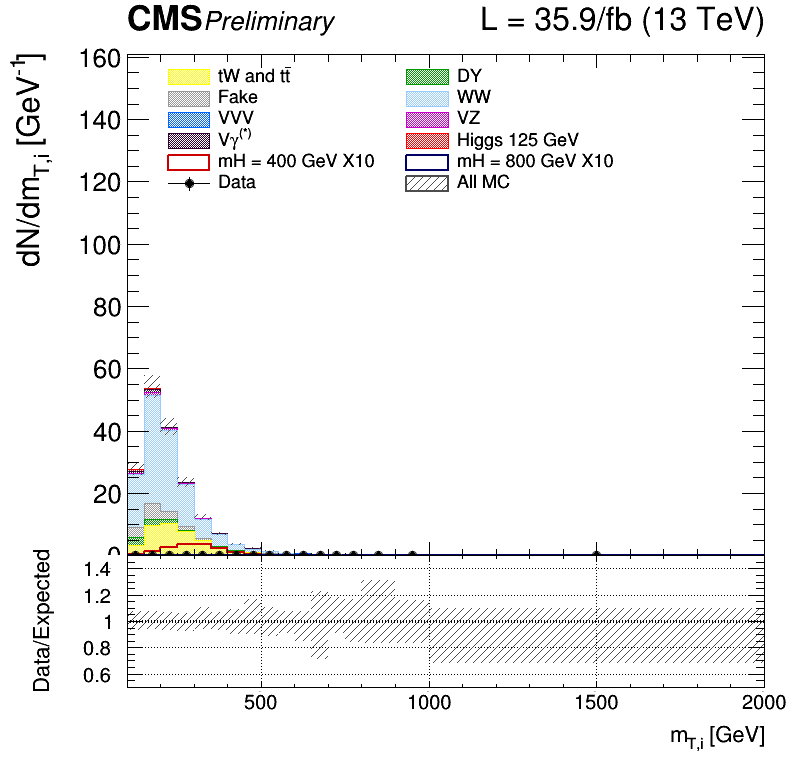
\includegraphics[width=0.45\textwidth]{Figs/OF_SR_Blind/cratio_hwwhm_13TeV_of_0j_mTi.png}
}
\subfigure[1 jet]{
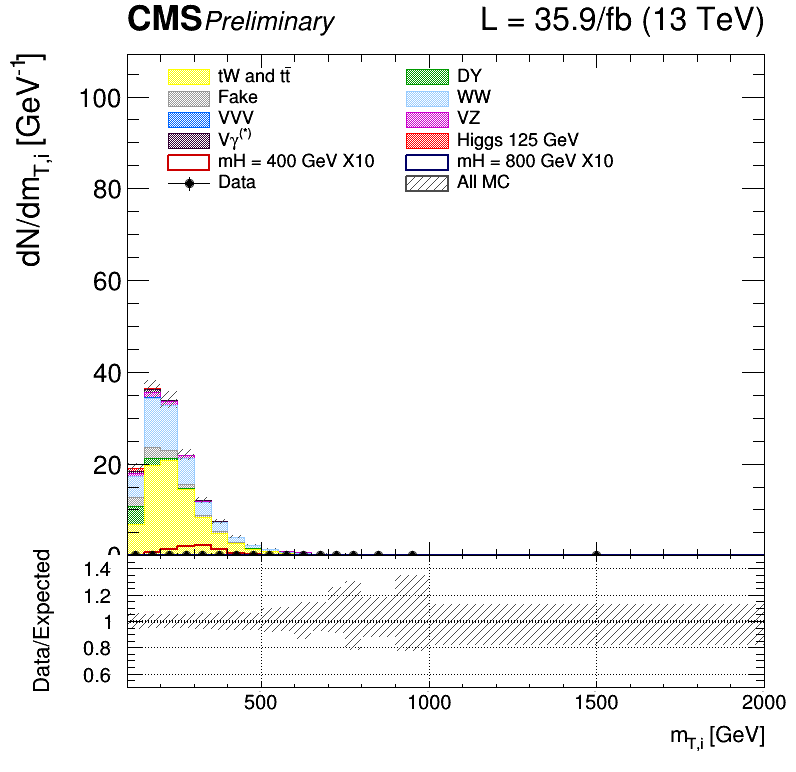
\includegraphics[width=0.45\textwidth]{Figs/OF_SR_Blind/cratio_hwwhm_13TeV_of_1j_mTi.png}
}
\\
\subfigure[2 jet]{
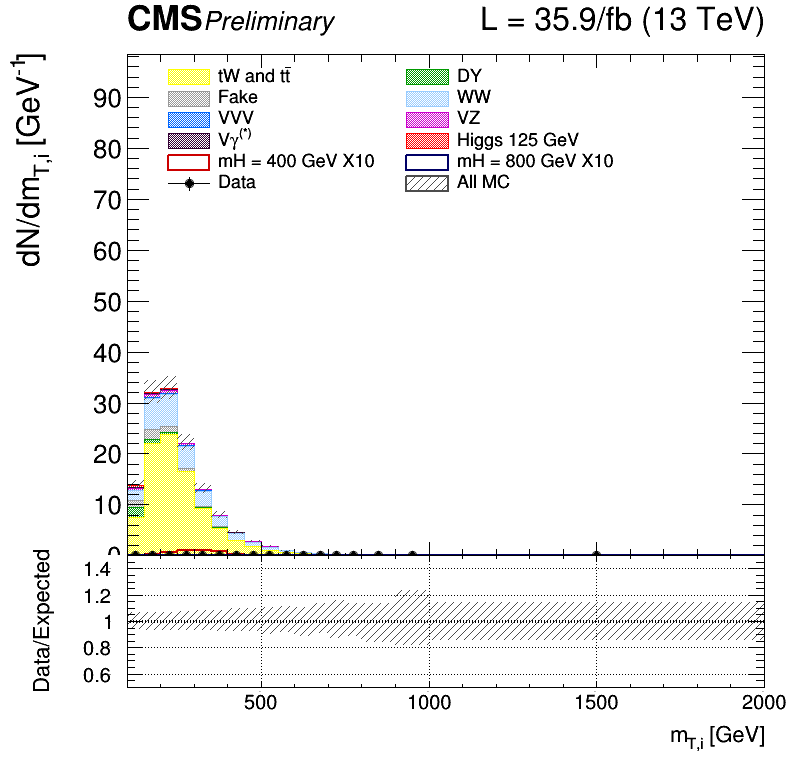
\includegraphics[width=0.45\textwidth]{Figs/OF_SR_Blind/cratio_hwwhm_13TeV_of2j_mTi.png}
}
\subfigure[VBF]{
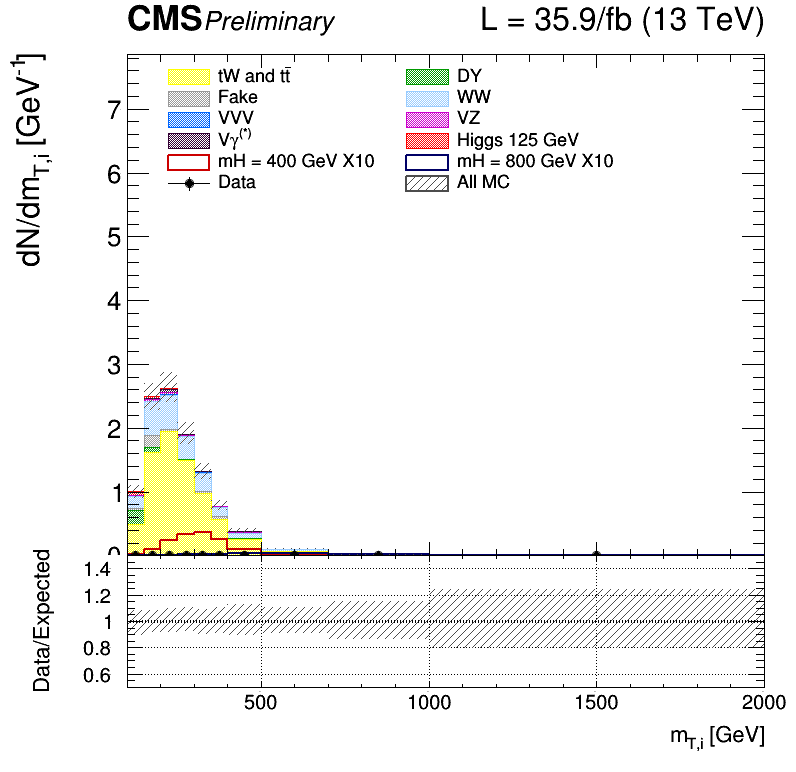
\includegraphics[width=0.45\textwidth]{Figs/OF_SR_Blind/cratio_hwwhm_13TeV_of_VBF_mTi_VBF.png}
}
\caption{Distributions  $m_T^I$ in the signal region for 0, 1, 2 and VBF categories. Two different signal hypothesis corresponding to $m_X $400 GeV and $m_X $800 GeV are shown superimposed to the background as a comparison. The binning is different in according to the number of jets.}
    \label{fig:mti_sigOF}
\end{figure}



\begin{figure}[htbp]
\centering
\subfigure[0 jet]{
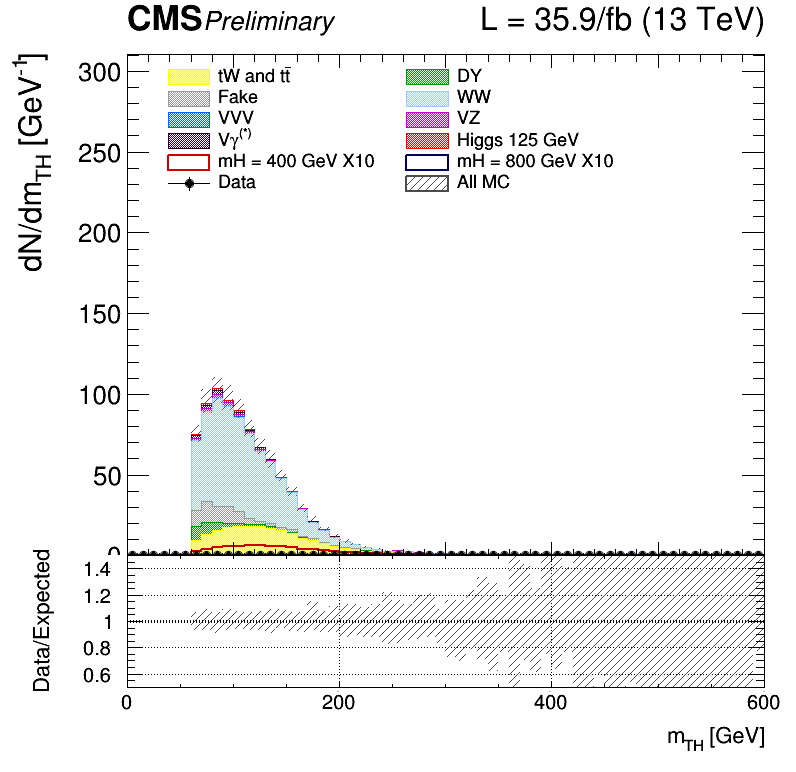
\includegraphics[width=0.45\textwidth]{Figs/OF_SR_Blind/cratio_hwwhm_13TeV_of_0j_mth.png}
}
\subfigure[1 jet]{
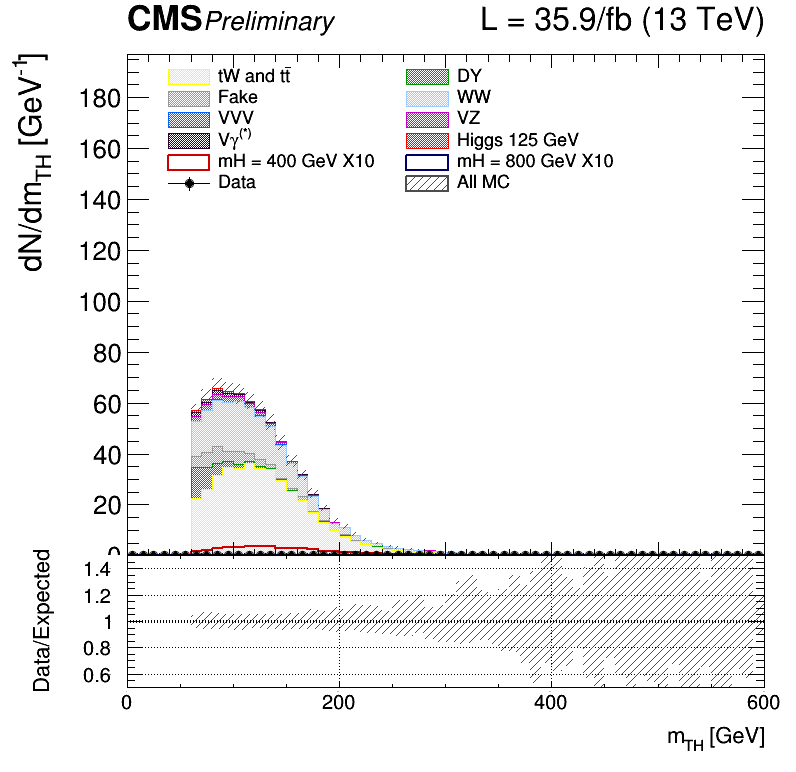
\includegraphics[width=0.45\textwidth]{Figs/OF_SR_Blind/cratio_hwwhm_13TeV_of_1j_mth.png}
}
\\
\subfigure[2 jet]{
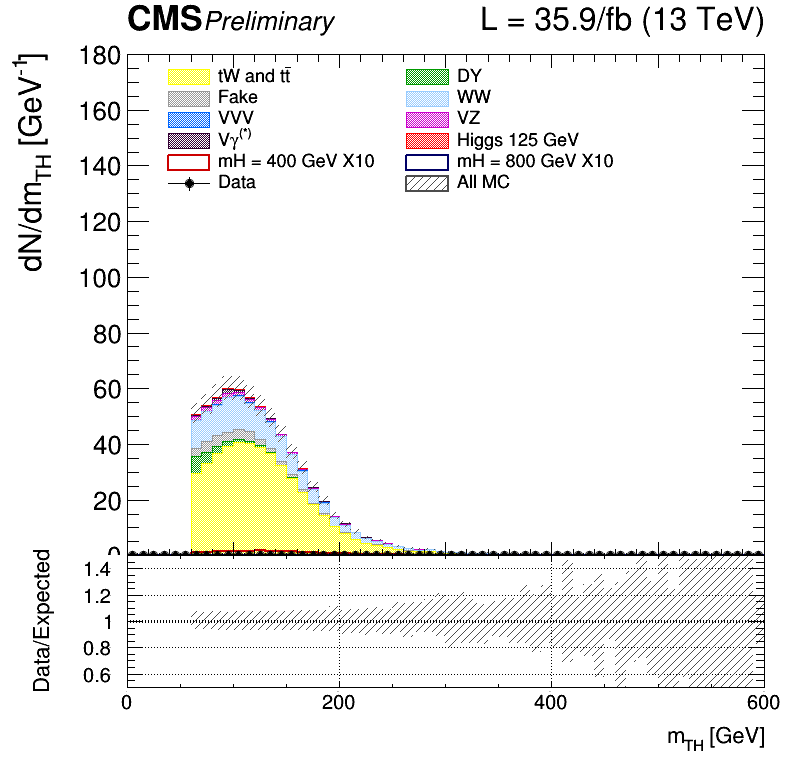
\includegraphics[width=0.45\textwidth]{Figs/OF_SR_Blind/cratio_hwwhm_13TeV_of2j_mth.png}
}
\subfigure[VBF]{
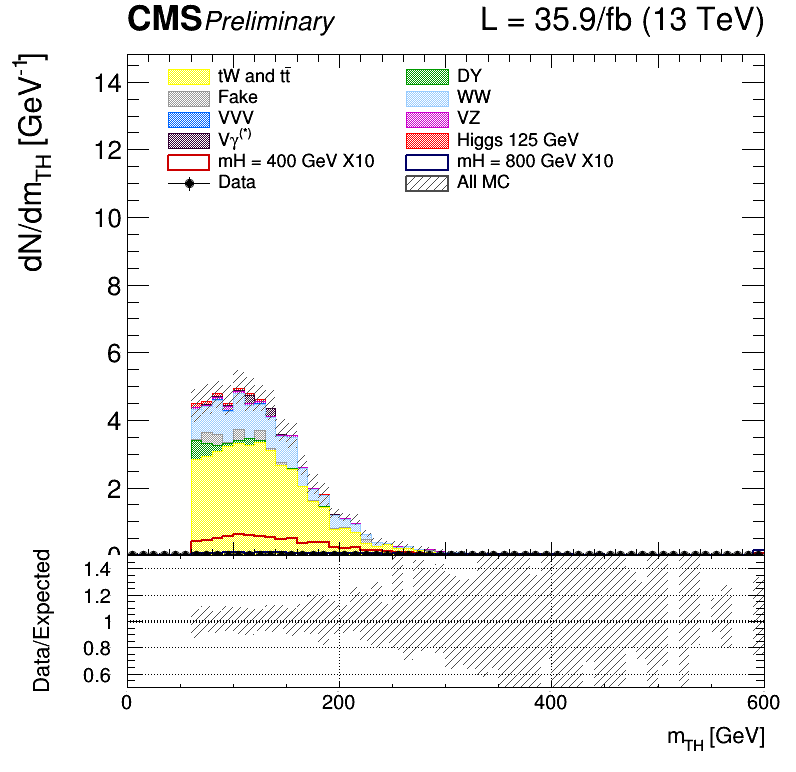
\includegraphics[width=0.45\textwidth]{Figs/OF_SR_Blind/cratio_hwwhm_13TeV_of_VBF_mth.png}
}
\caption{Distributions  $m_T^H$ in the signal region for 0, 1, 2 and VBF categories. Two different signal hypothesis corresponding to $m_X $400 GeV and $m_X $800 GeV are shown superimposed to the background as a comparison. The binning for  $m_T^H$ is the same in the jets categories.}
    \label{fig:mth_sigOF}
\end{figure}



\begin{figure}[htbp]
\centering
\subfigure[0 jet]{
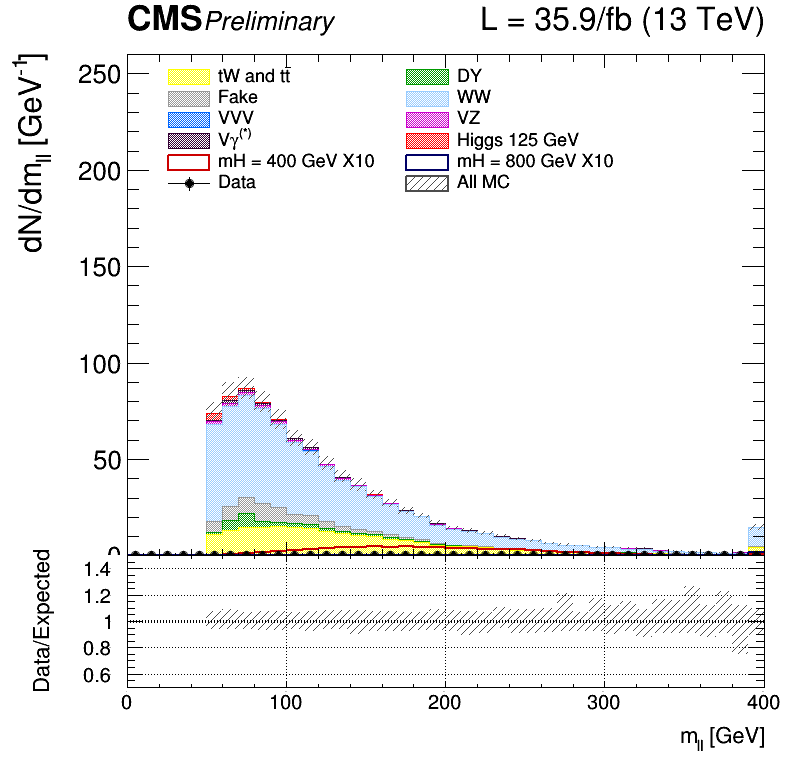
\includegraphics[width=0.45\textwidth]{Figs/OF_SR_Blind/cratio_hwwhm_13TeV_of_0j_mll.png}
}
\subfigure[1 jet]{
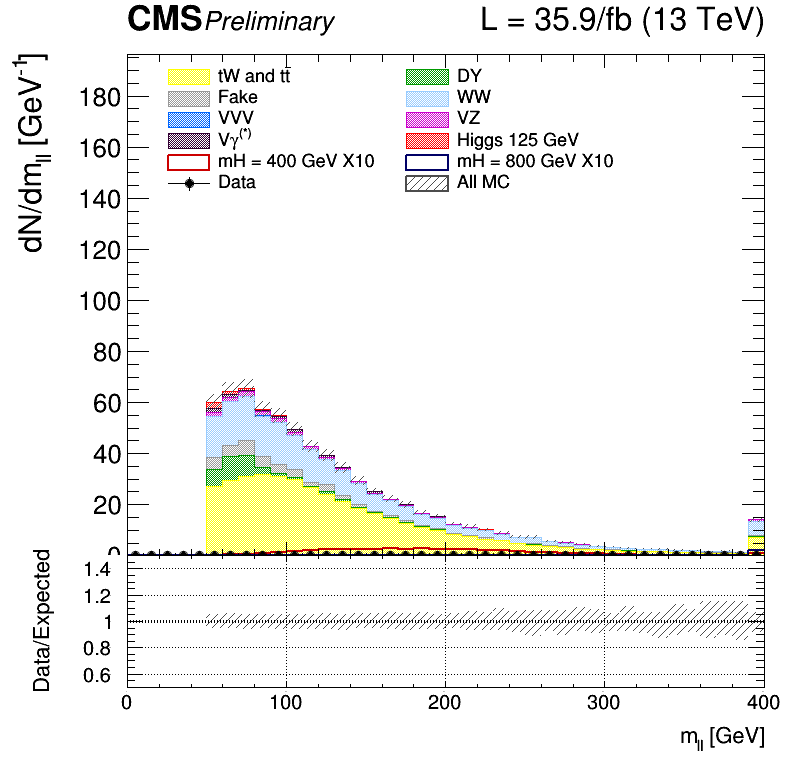
\includegraphics[width=0.45\textwidth]{Figs/OF_SR_Blind/cratio_hwwhm_13TeV_of_1j_mll.png}
}
\\
\subfigure[2 jet]{
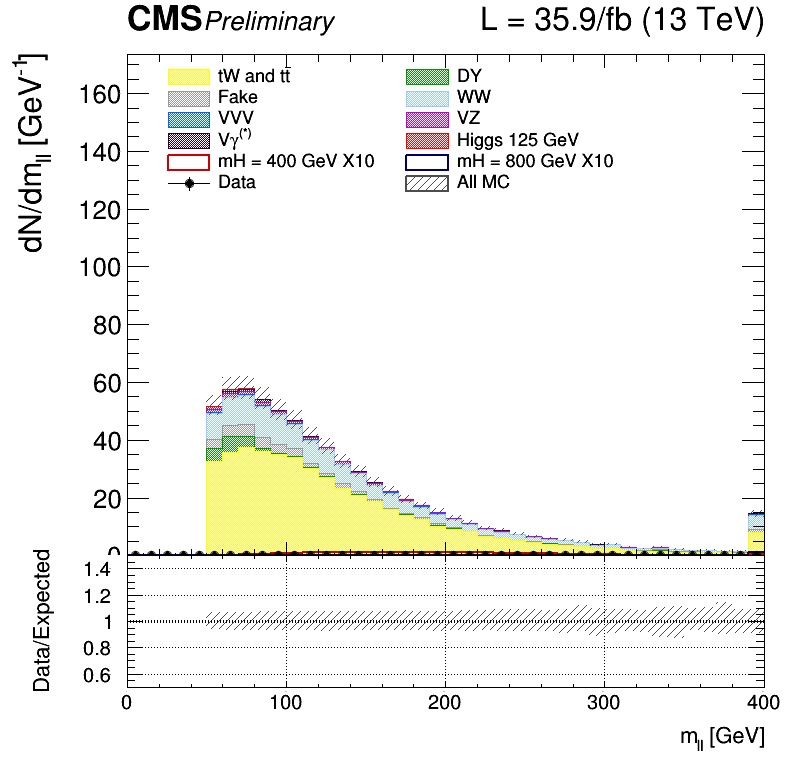
\includegraphics[width=0.45\textwidth]{Figs/OF_SR_Blind/cratio_hwwhm_13TeV_of2j_mll.png}
}
\subfigure[VBF]{
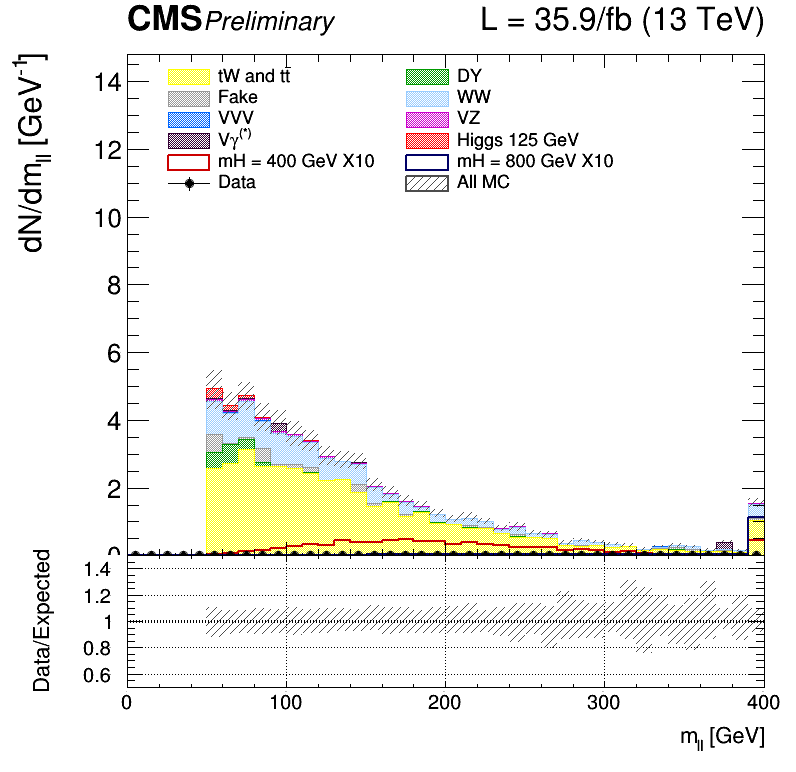
\includegraphics[width=0.45\textwidth]{Figs/OF_SR_Blind/cratio_hwwhm_13TeV_of_VBF_mll.png}
}
\caption{Distributions  $m_{\ell \ell}$ in the signal region for 0, 1, 2 and VBF categories. Two different signal hypothesis corresponding to $m_X $400 GeV and $m_X $800 GeV are shown superimposed to the background as a comparison. The binning for $m_{\ell \ell}$ is the same in the jets categories.}
    \label{fig:mll_sigOF}
\end{figure}


The different contributin of the signal,   the gluon-gluon fusion, the VBS and the interferences
are shown separately in Fig.~\ref{fig:mti_Diff_contrib400}  for the $m_T^I$ distribution .  %and Fig.~\ref{fig:mti_Diff_contrib2000}



\begin{figure}[htbp]
\centering
\subfigure[0 jet]{
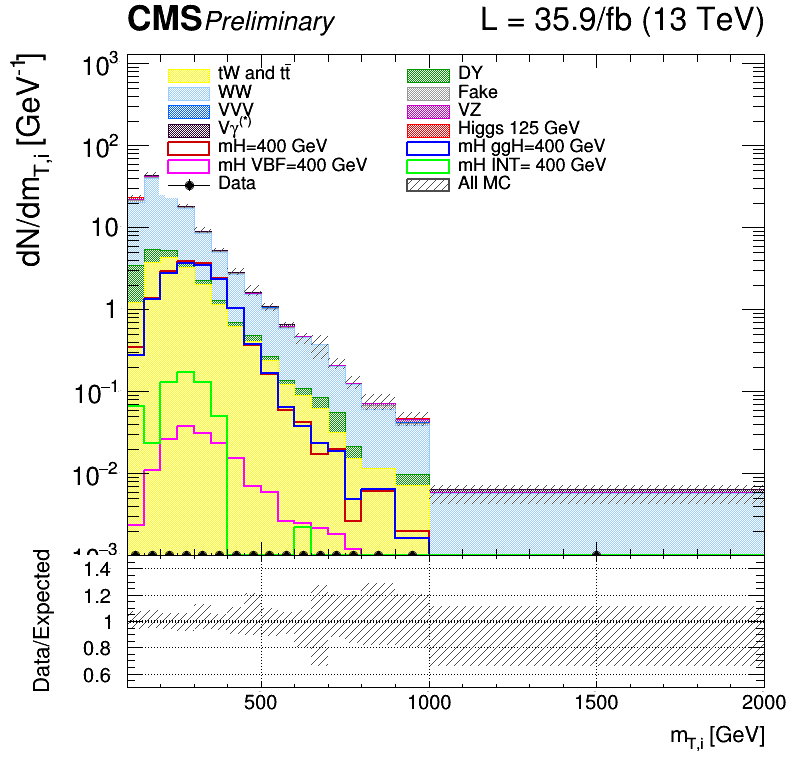
\includegraphics[width=0.45\textwidth]{Figs/OF_SR_sep_contrib/400/log_cratio_hwwhm_13TeV_of0j_mTi.png}
}
\subfigure[1 jet]{
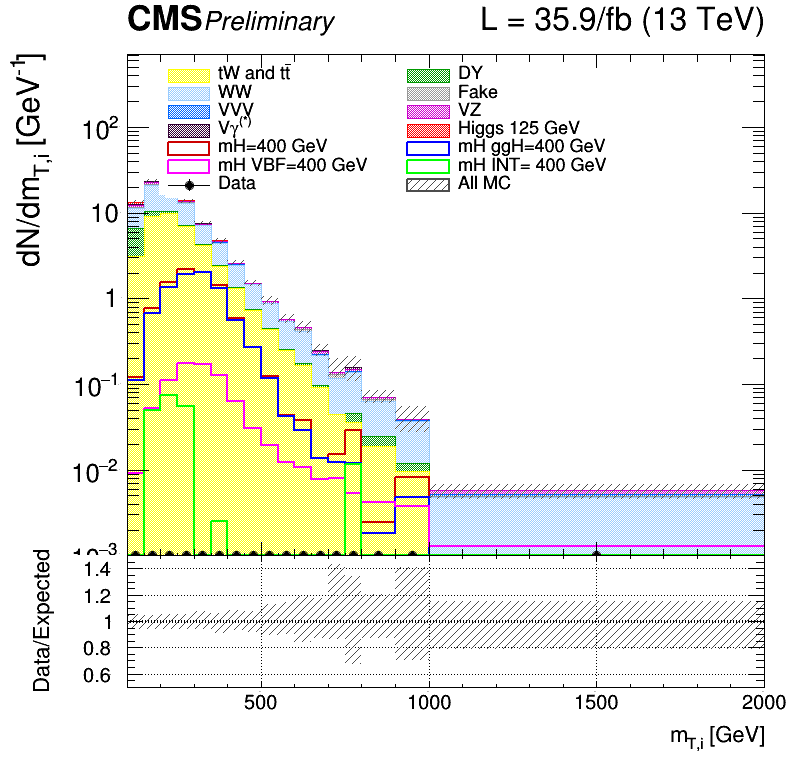
\includegraphics[width=0.45\textwidth]{Figs/OF_SR_sep_contrib/400/log_cratio_hwwhm_13TeV_of1j_mTi.png}
}
\\
\subfigure[2 jet]{
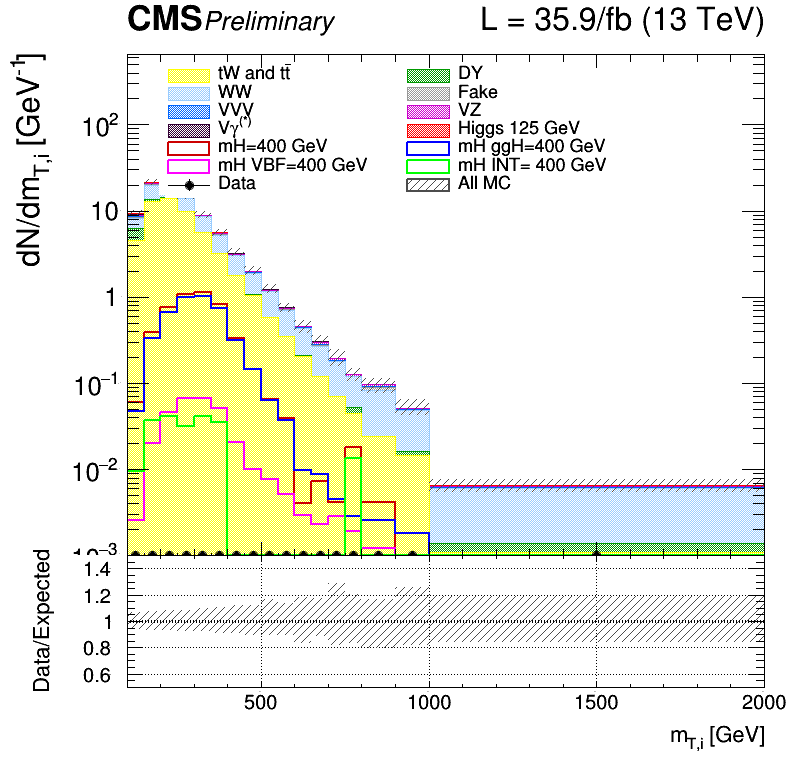
\includegraphics[width=0.45\textwidth]{Figs/OF_SR_sep_contrib/400/log_cratio_hwwhm_13TeV_of2j_mTi.png}
}
\subfigure[VBF]{
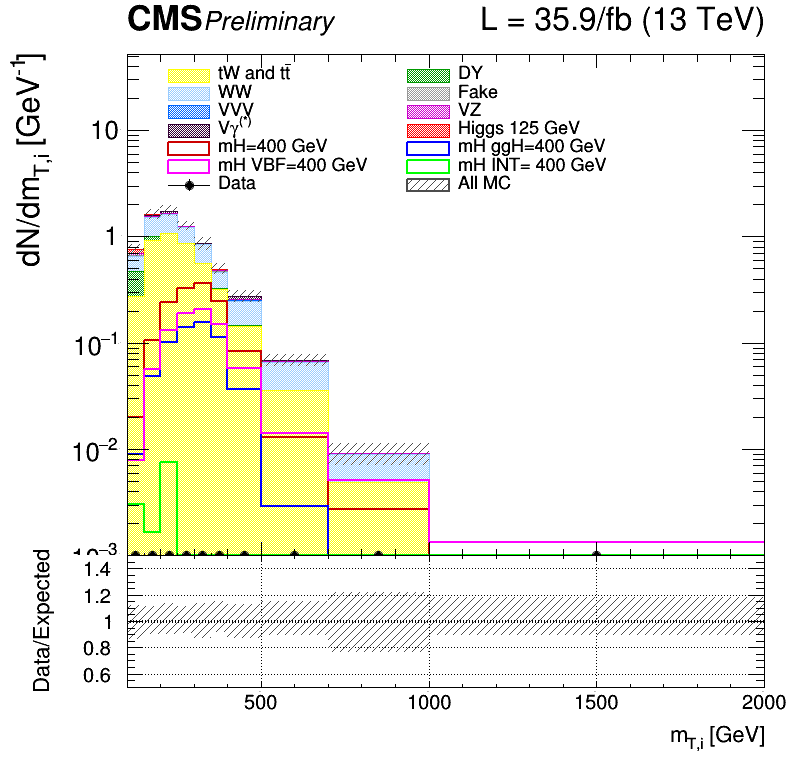
\includegraphics[width=0.45\textwidth]{Figs/OF_SR_sep_contrib/400/log_cratio_hwwhm_13TeV_ofVBF_mTi_VBF.png}
}
\caption{Distributions of the different contribution of the signal for  $m_T^I$ in region for 0, 1, 2 and VBF categories. The  signal hypothesis corresponding to $m_X $400. The red line correspond to the Signal (total), the blue line correspond to the gluon-gluon contribution, the violet correspond to the VBF and the green to to total (gluon-gluon+VBF) interference.}
    \label{fig:mti_Diff_contrib400}
\end{figure}




%\begin{figure}[htbp]
%\centering
%\subfigure[0 jet]{
%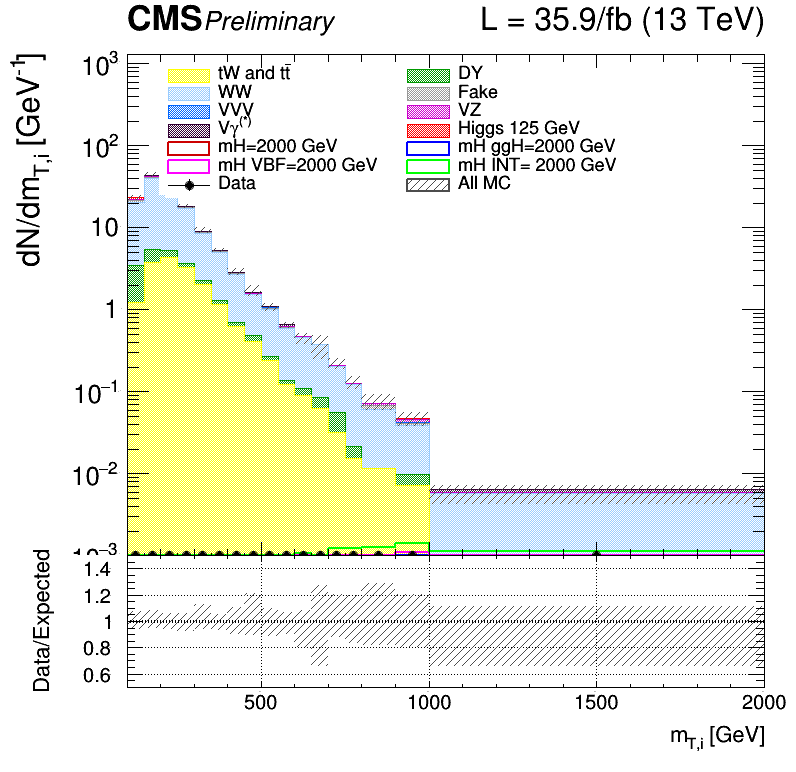
\includegraphics[width=0.45\textwidth]{Figs/OF_SR_sep_contrib/2000/log_cratio_hwwhm_13TeV_of0j_mTi.png}
%}
%\subfigure[1 jet]{
%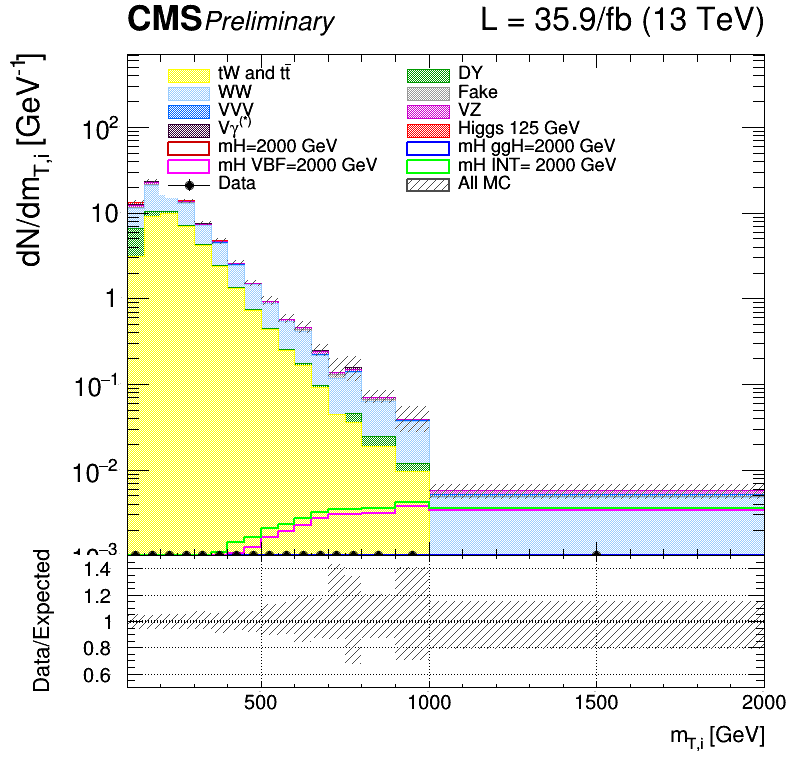
\includegraphics[width=0.45\textwidth]{Figs/OF_SR_sep_contrib/2000/log_cratio_hwwhm_13TeV_of1j_mTi.png}
%}
%\\
%\subfigure[2 jet]{
%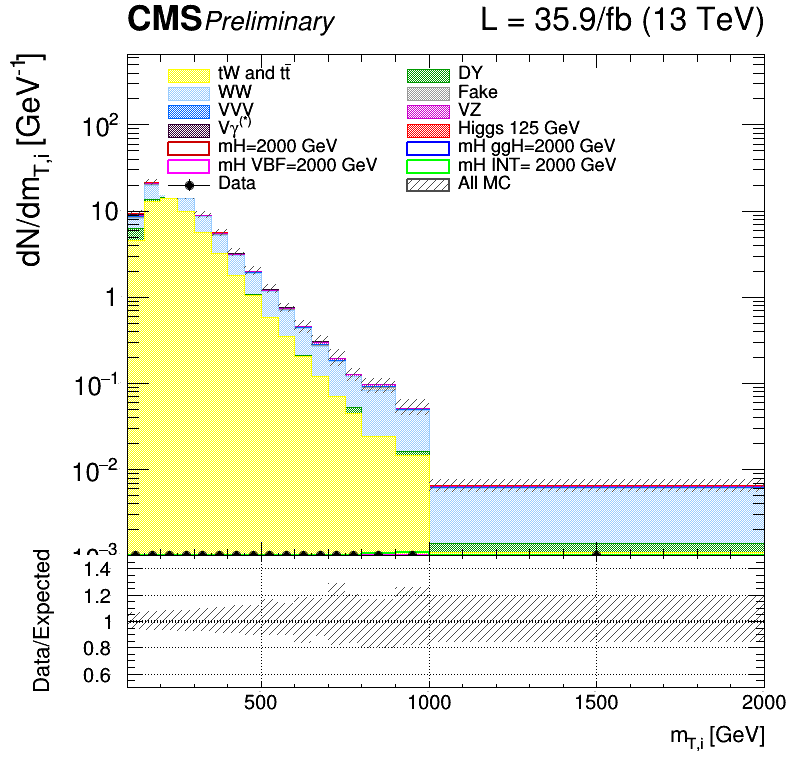
\includegraphics[width=0.45\textwidth]{Figs/OF_SR_sep_contrib/2000/log_cratio_hwwhm_13TeV_of2j_mTi.png}
%}
%\subfigure[VBF]{
%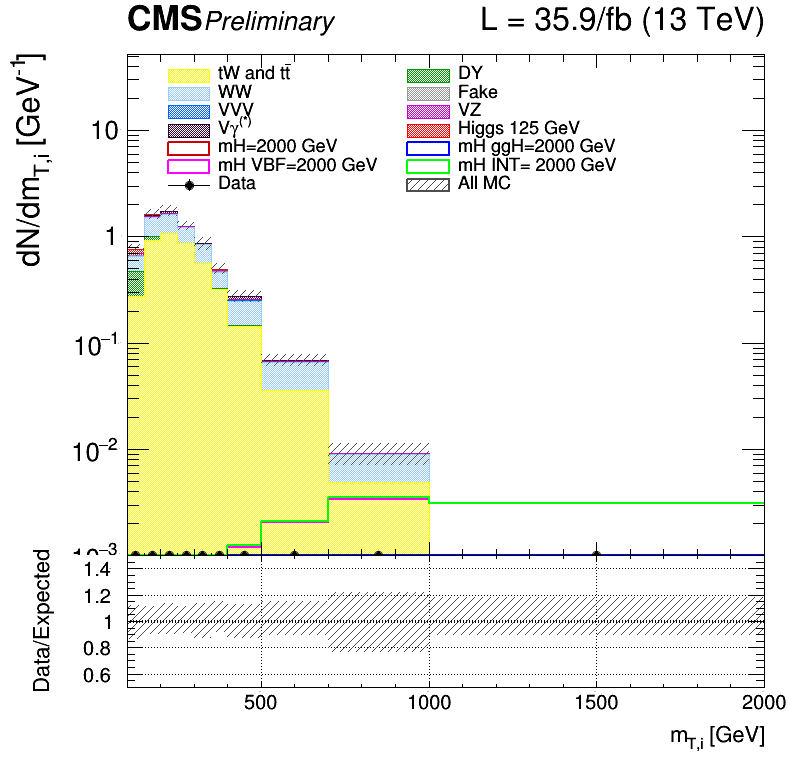
\includegraphics[width=0.45\textwidth]{Figs/OF_SR_sep_contrib/2000/log_cratio_hwwhm_13TeV_ofVBF_mTi_VBF.png}
%}
%\caption{Distributions of the different contribution of the signal for  $m_T^I$ in region for 0, 1, 2 and VBF categories. The  signal hypothesis corresponding to $m_X $ 2000. The red line correspond to the Signal (total), the blue line correspond to the gluon-gluon contribution, the violet correspond to the VBF and the green to to total (gluon-gluon+VBF) interference.}
%    \label{fig:mti_Diff_contrib2000}
%\end{figure}


\subsection{Signal region Unblinding}
The unblinding  $m_T^I$ distribution of the signal regions is shown is Fig. \ref{fig:mti_sigOF_Un} and Fig. \ref{fig:mti_sigOF_Un_log} 

\begin{figure}[htbp]
\centering
\subfigure[0 jet]{
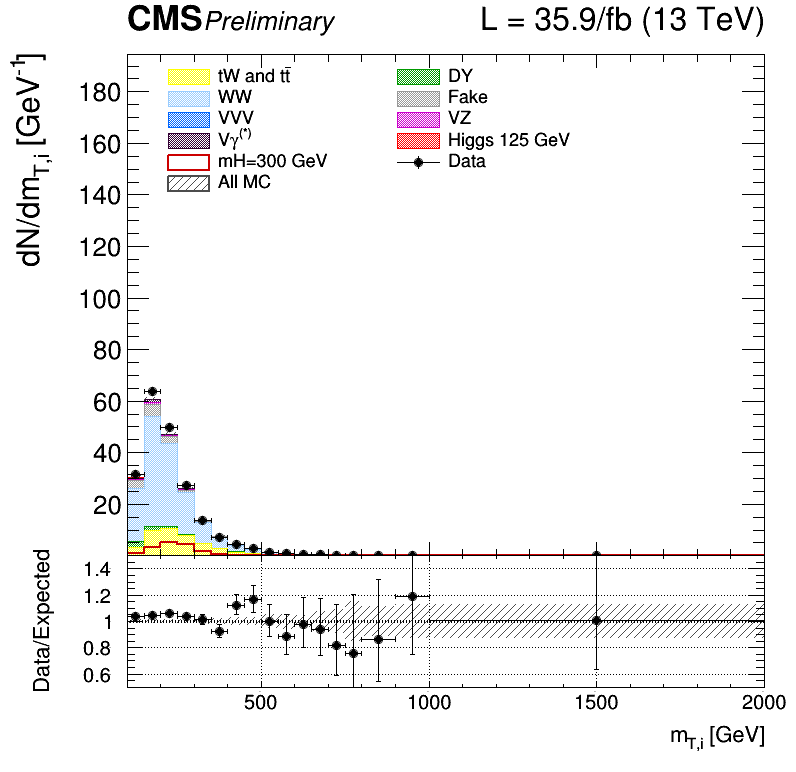
\includegraphics[width=0.45\textwidth]{Figs/unblinding/plot_SR/plotHWWhighMass_OF_300_postFit_0j/cratio_hwwhm_13TeV_of0j_mTi.png}
}
\subfigure[1 jet]{
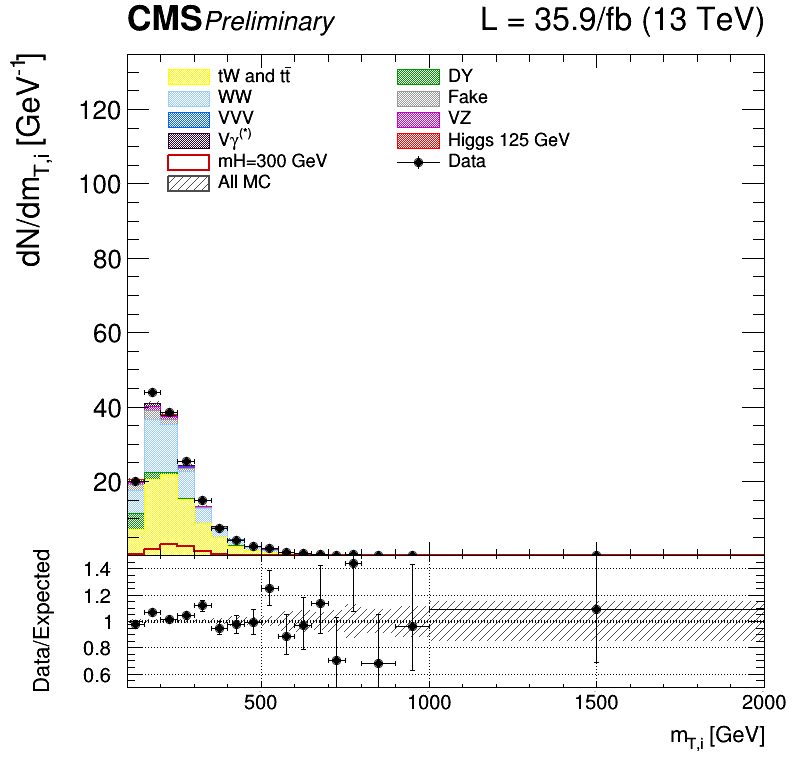
\includegraphics[width=0.45\textwidth]{Figs/unblinding/plot_SR/plotHWWhighMass_OF_300_postFit_1j/cratio_hwwhm_13TeV_of1j_mTi.png}
}
\\
\subfigure[2 jet]{
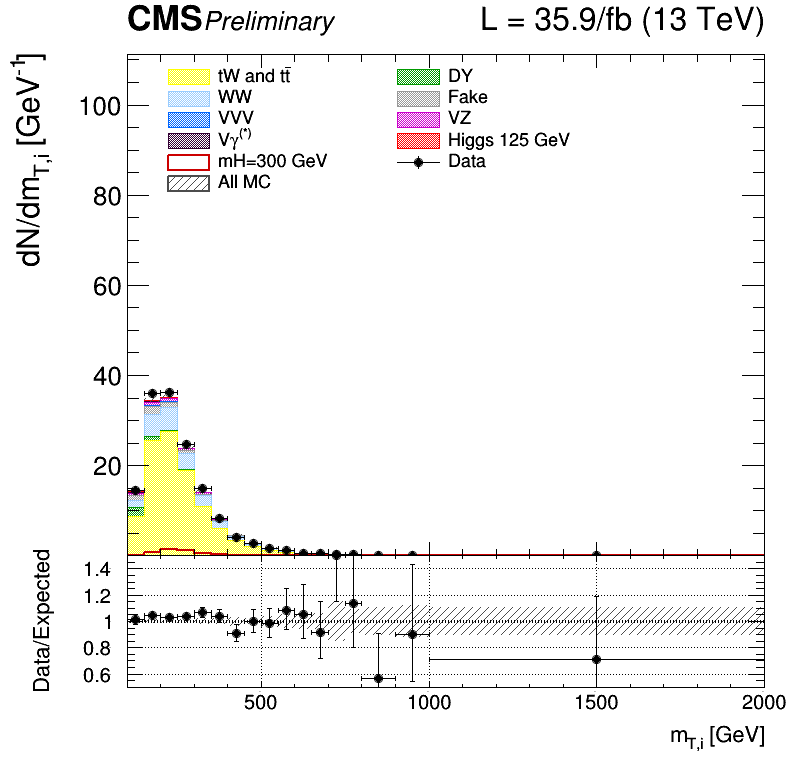
\includegraphics[width=0.45\textwidth]{Figs/unblinding/plot_SR/plotHWWhighMass_OF_300_postFit_2j/cratio_hwwhm_13TeV_of2j_mTi.png}
}
\subfigure[VBF]{
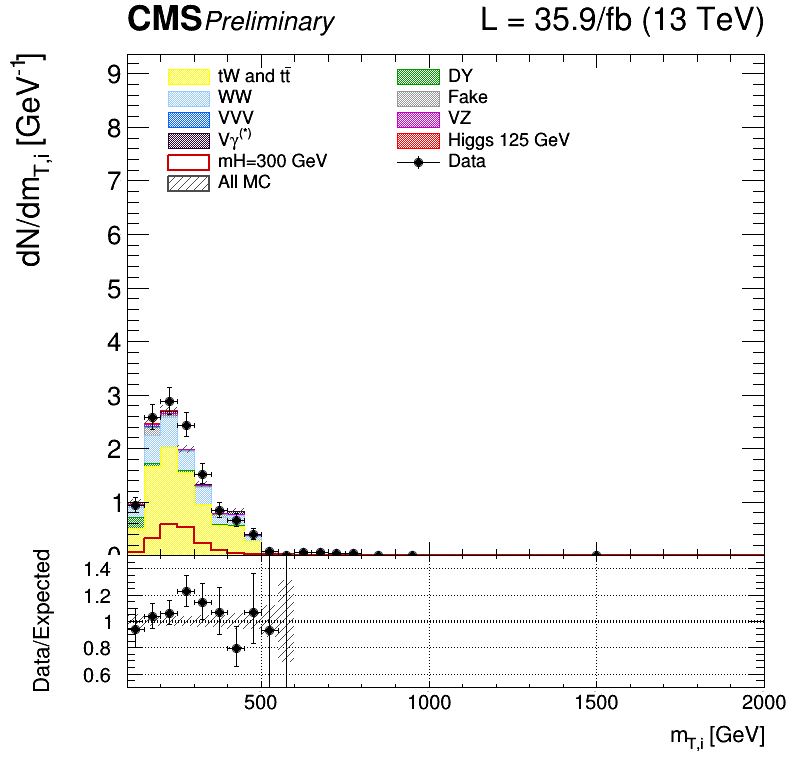
\includegraphics[width=0.45\textwidth]{Figs/unblinding/plot_SR/plotHWWhighMass_OF_300_postFit_VBF/cratio_hwwhm_13TeV_ofVBF_mTi.png}
}
\caption{Unblinding distributions  $m_T^I$ in the signal region for 0, 1, 2 and VBF categories. The signal hypothesis corresponding to $m_X $ of 300 GeV.}
    \label{fig:mti_sigOF_Un}
\end{figure}


\begin{figure}[htbp]
\centering
\subfigure[0 jet]{
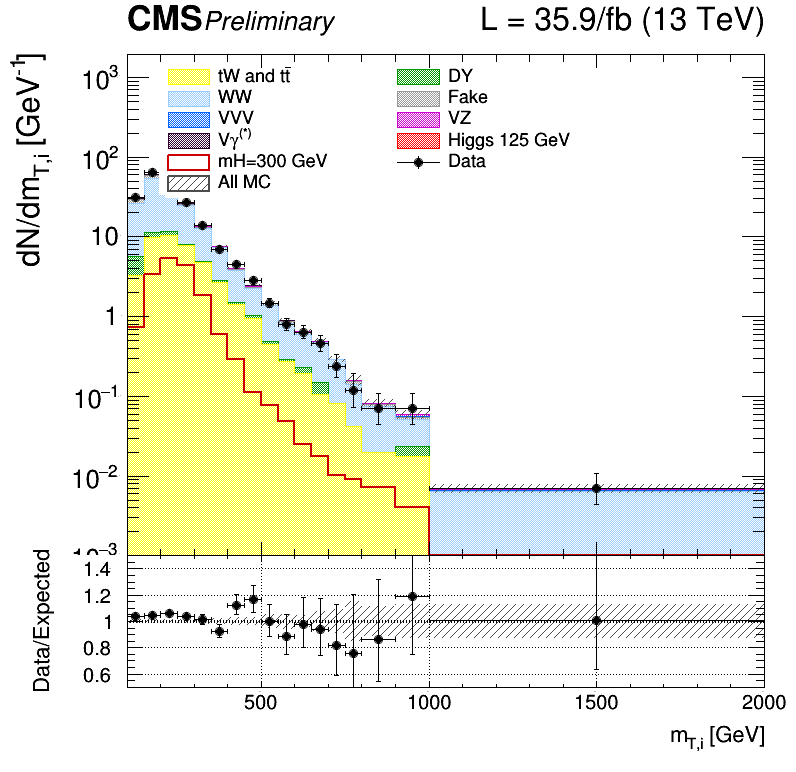
\includegraphics[width=0.45\textwidth]{Figs/unblinding/plot_SR/plotHWWhighMass_OF_300_postFit_0j/log_cratio_hwwhm_13TeV_of0j_mTi.png}
}
\subfigure[1 jet]{
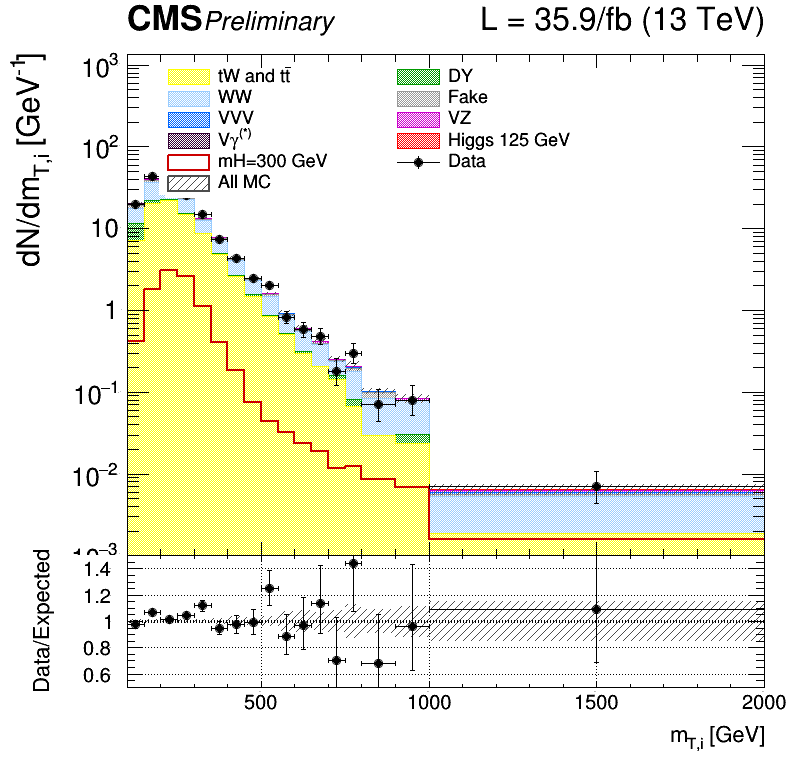
\includegraphics[width=0.45\textwidth]{Figs/unblinding/plot_SR/plotHWWhighMass_OF_300_postFit_1j/log_cratio_hwwhm_13TeV_of1j_mTi.png}
}
\\
\subfigure[2 jet]{
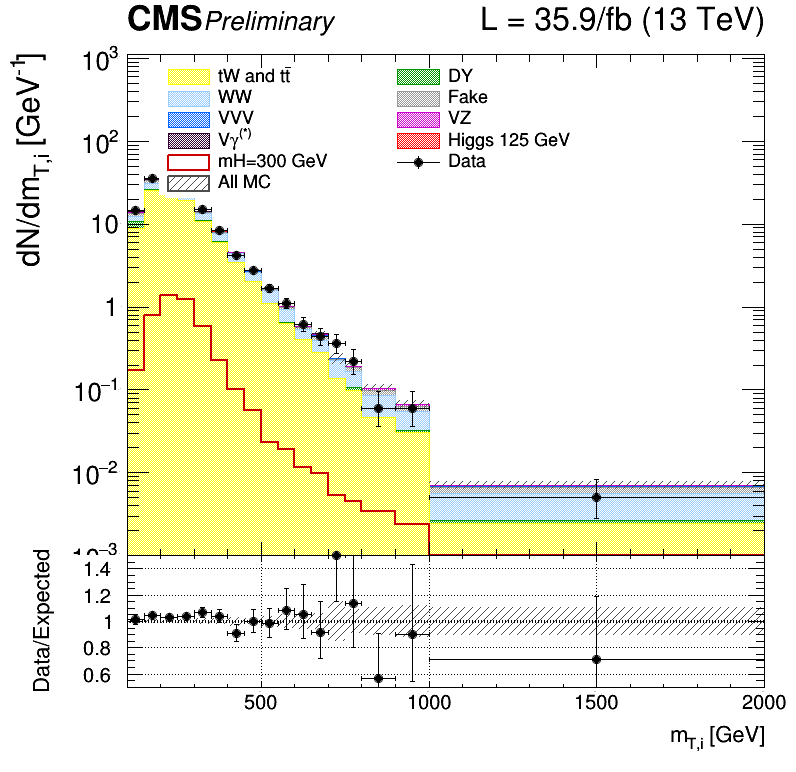
\includegraphics[width=0.45\textwidth]{Figs/unblinding/plot_SR/plotHWWhighMass_OF_300_postFit_2j/log_cratio_hwwhm_13TeV_of2j_mTi.png}
}
\subfigure[VBF]{
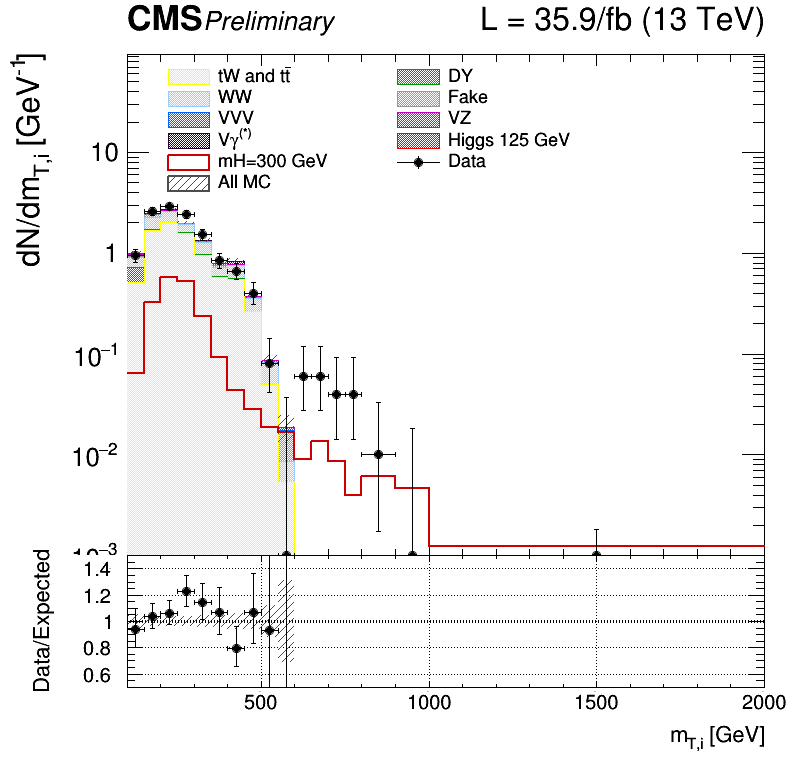
\includegraphics[width=0.45\textwidth]{Figs/unblinding/plot_SR/plotHWWhighMass_OF_300_postFit_VBF/log_cratio_hwwhm_13TeV_ofVBF_mTi.png}
}
\caption{Unblinding distributions  $m_T^I$ in the signal region for 0, 1, 2 and VBF categories. The signal hypothesis corresponding to $m_X $ of 300 GeV.}
    \label{fig:mti_sigOF_Un_log}
\end{figure}






\subsection{Background estimation}
The main background processes that affect this signature arise from non-resonant WW production and from top production, including tt pairs and single top production (mostly tW), and are estimated using data. Instrumental backgrounds arising from non-prompt leptons in
W+jets production and mis-measurement of $E_T^{miss}$ in Drell-Yan events are also estimated from
data. The contribution from W$\gamma^*$  is estimated partly from data. The
contribution of other sub-dominant backgrounds is obtained directly from simulated samples. The different data-driven background estimations are explained in the following subsections.\\
\newline
More precisely top and DY backgrounds normalizations have been extracted
directly from
data-simulation comparison in specific control regions enriched in either one
or the other background separately for the 0, 1 ,2 and VBF jet categories, using the rateParam feature of the combine package.


\subsection{Drell-Yan $\tau\tau$ control region}
To normalize the Drell-Yan $\tau\tau$ background to the data, control regions
have been defined, as close as possible to the signal region, but enriched in
Z $\rightarrow \tau^+ \tau^-$. In particular, the WW OF selection is used with
inverted $m_T^H$ cut, i.e. $m_T^H<60$. In addition a cut on the invariant mass
of the two leptons 50 GeV $< m_{\ell \ell} <$ 80 GeV is requested to exclude
possible contribution from non-prompt leptons (low limit) and from tt (high
limit).

For each signal category, a corresponding Drell-Yan $\tau\tau$ control
regions is defined. We thus have 4 total  Drell-Yan $\tau\tau$ control
regions, for 0 jets, 1 jets, 2 jets and VBF.

The control plots for several variables in a Drell-Yan enriched phase space
for the four jets categories are shown in Figs.~\ref{fig:CR_DY_OF_0},
~\ref{fig:CR_DY_OF_1}, ~\ref{fig:CR_DY_OF_2}, ~\ref{fig:CR_DY_OF_VBF}.
In general there is a good agreement between data and MC.\\

\begin{figure}[htbp]
\centering
\subfigure[$m_T^I$]{
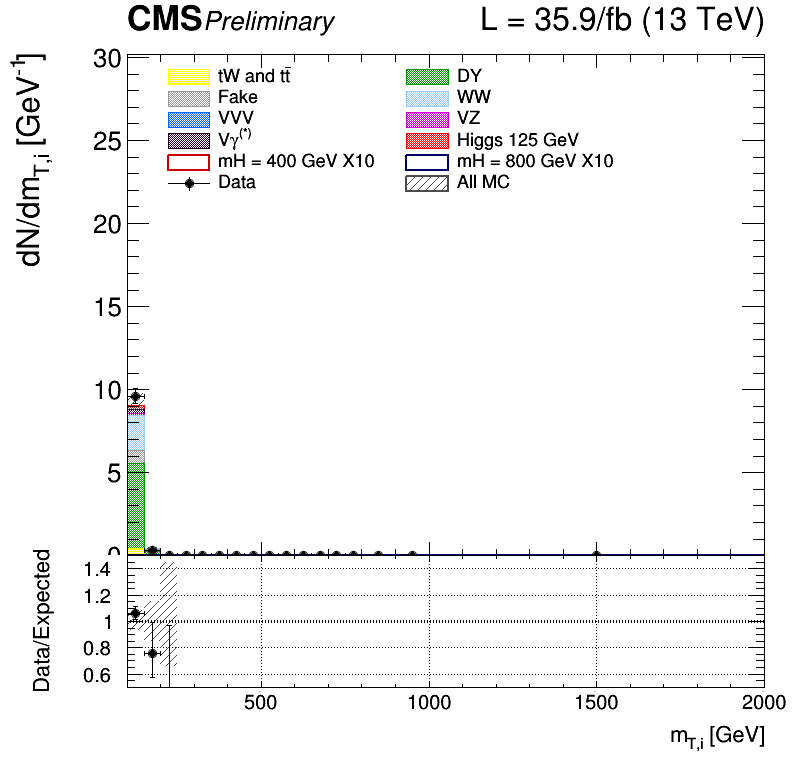
\includegraphics[width=0.45\textwidth]{Figs/OF_CR_Blind/cratio_hww2l2v_13TeV_dytt_of0j_mTi.png}
}
\subfigure[$m_T^H$]{
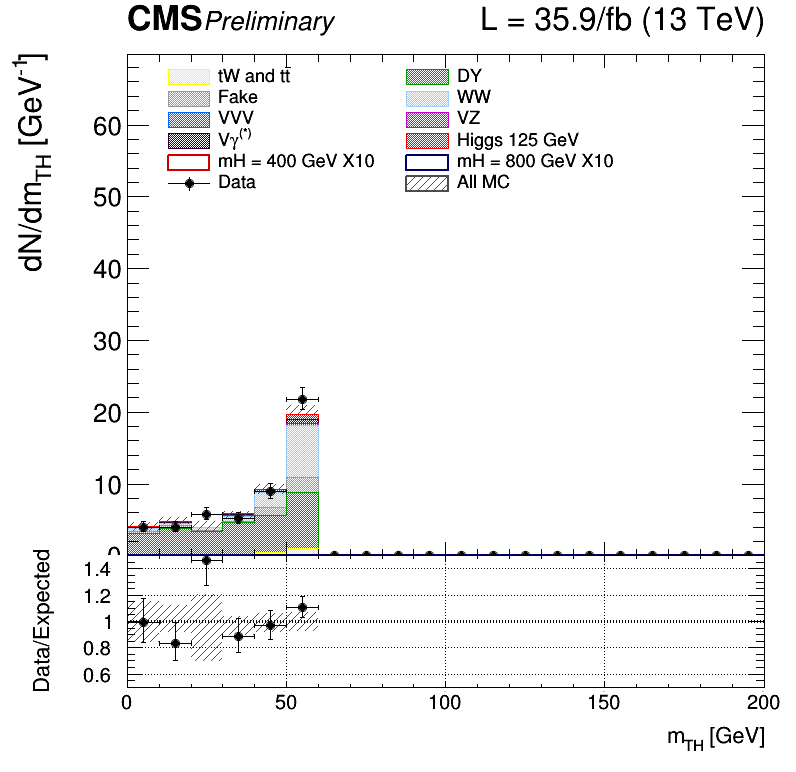
\includegraphics[width=0.45\textwidth]{Figs/OF_CR_Blind/cratio_hww2l2v_13TeV_dytt_of0j_mth_DY.png}
}                                              
\\                                             
\subfigure[$m_{jj}$]{                             
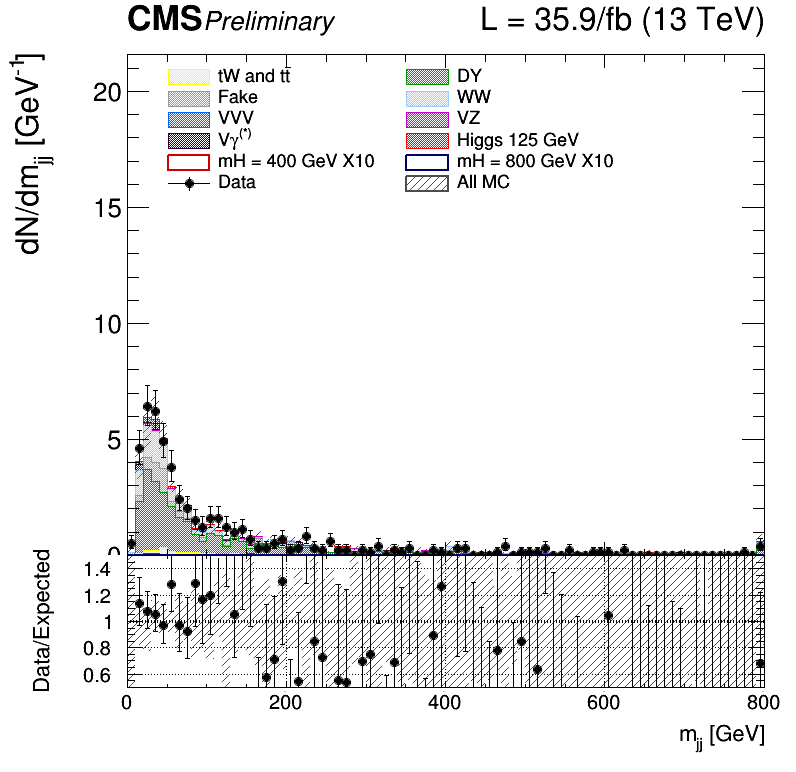
\includegraphics[width=0.45\textwidth]{Figs/OF_CR_Blind/cratio_hww2l2v_13TeV_dytt_of0j_mjj.png}
}                                              
\subfigure[$m_{\ell \ell}$]{                               
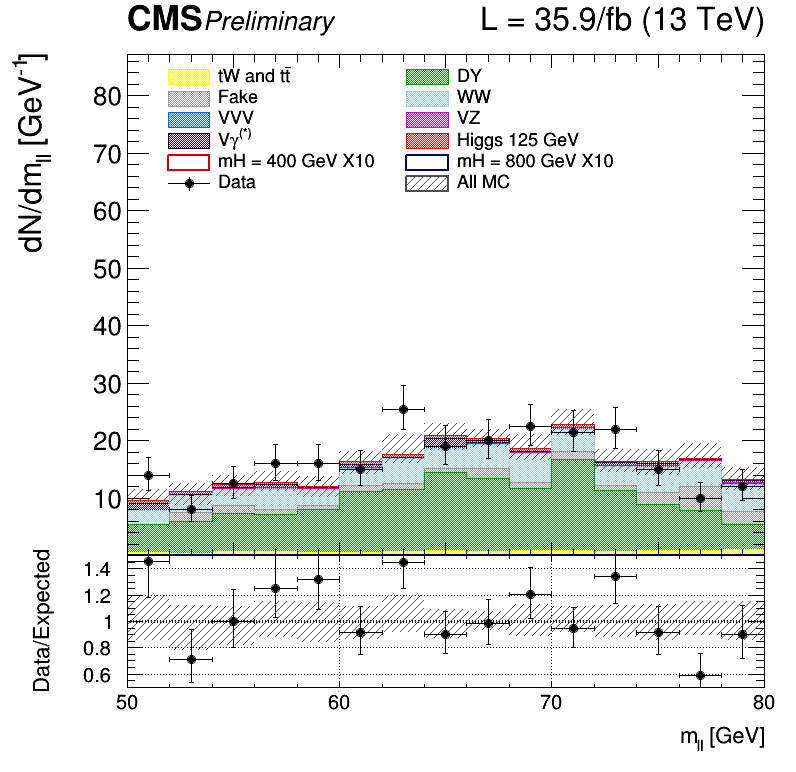
\includegraphics[width=0.45\textwidth]{Figs/OF_CR_Blind/cratio_hww2l2v_13TeV_dytt_of0j_mll_DY.png}
}\\

\subfigure[$p_T$ leading lepton]{                             
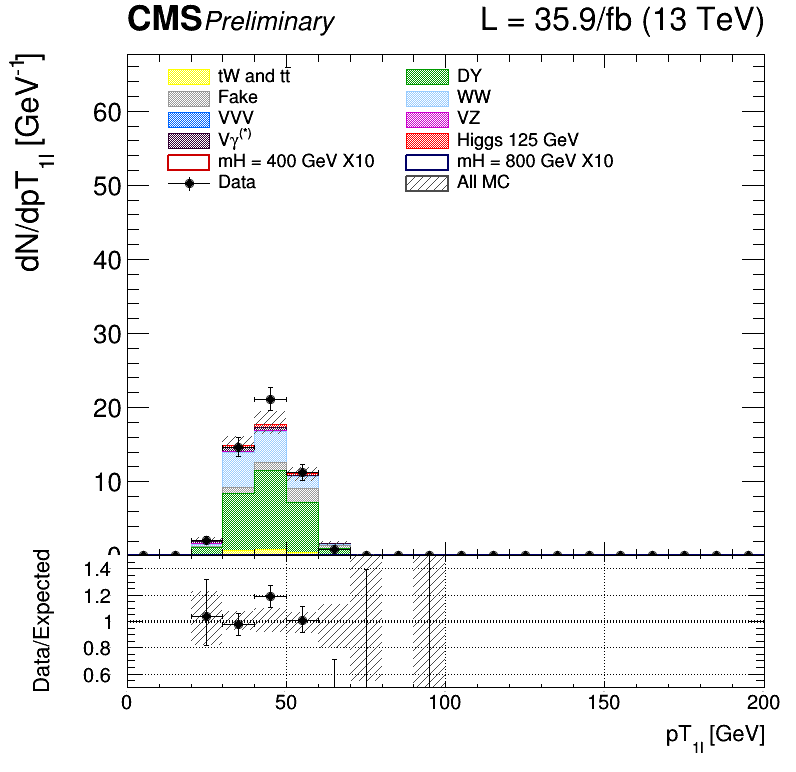
\includegraphics[width=0.45\textwidth]{Figs/OF_CR_Blind/cratio_hww2l2v_13TeV_dytt_of0j_std_vector_lepton_pt[0].png}
}                                              
\subfigure[$p_T^{\ell \ell}$]{                               
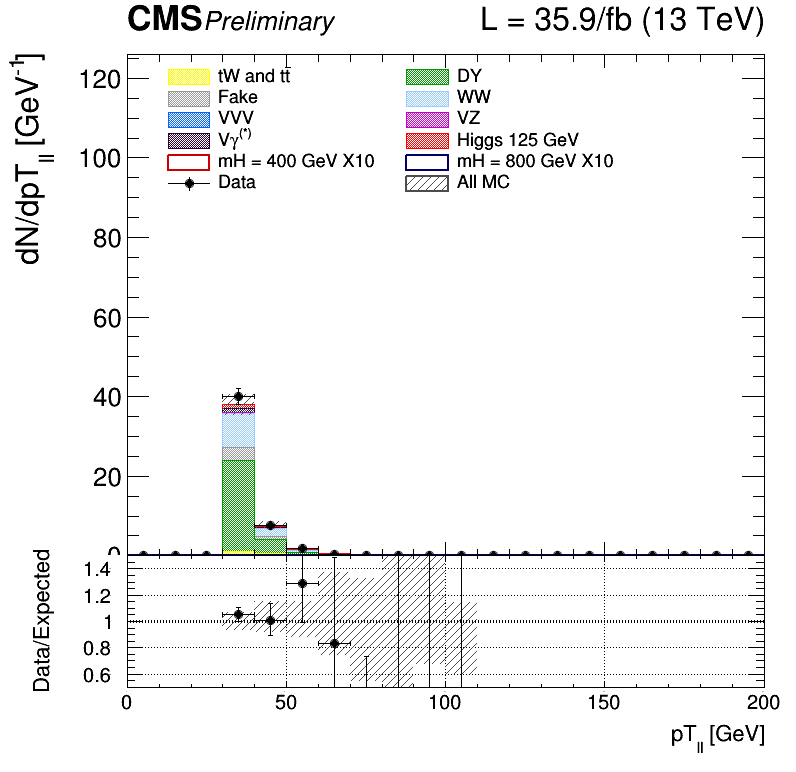
\includegraphics[width=0.45\textwidth]{Figs/OF_CR_Blind/cratio_hww2l2v_13TeV_dytt_of0j_ptll.png}
}\\

\caption{Control plots for several variables in a Drell-Yan enriched phase space for events with 0 jet.}
    \label{fig:CR_DY_OF_0}
\end{figure}





\begin{figure}[htbp]
\centering
\subfigure[$m_T^I$]{
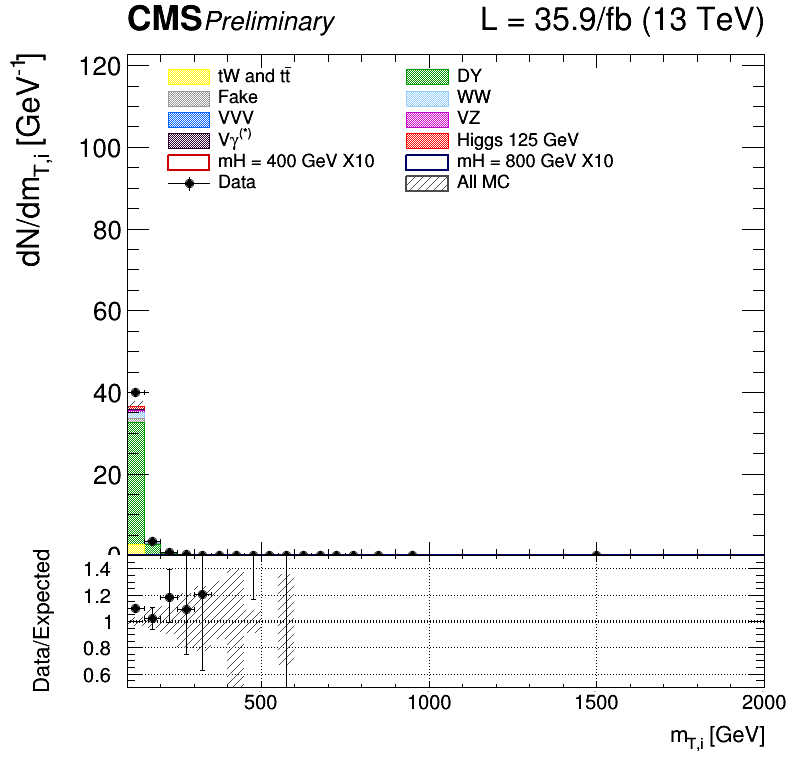
\includegraphics[width=0.45\textwidth]{Figs/OF_CR_Blind/cratio_hww2l2v_13TeV_dytt_of1j_mTi.png}
}
\subfigure[$m_T^H$]{
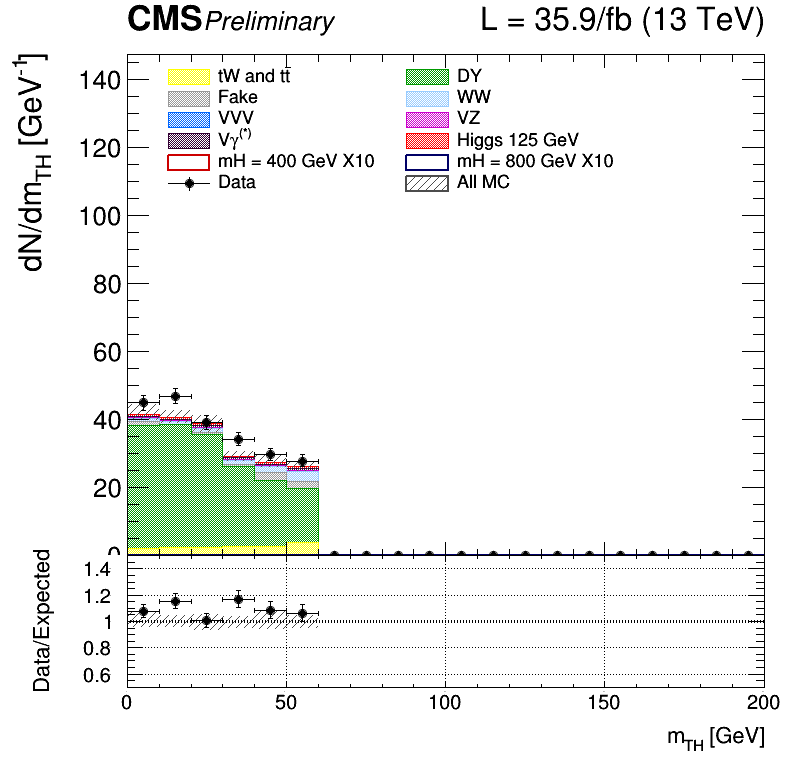
\includegraphics[width=0.45\textwidth]{Figs/OF_CR_Blind/cratio_hww2l2v_13TeV_dytt_of1j_mth_DY.png}
}                                              
\\                                             
\subfigure[$m_{jj}$]{                             
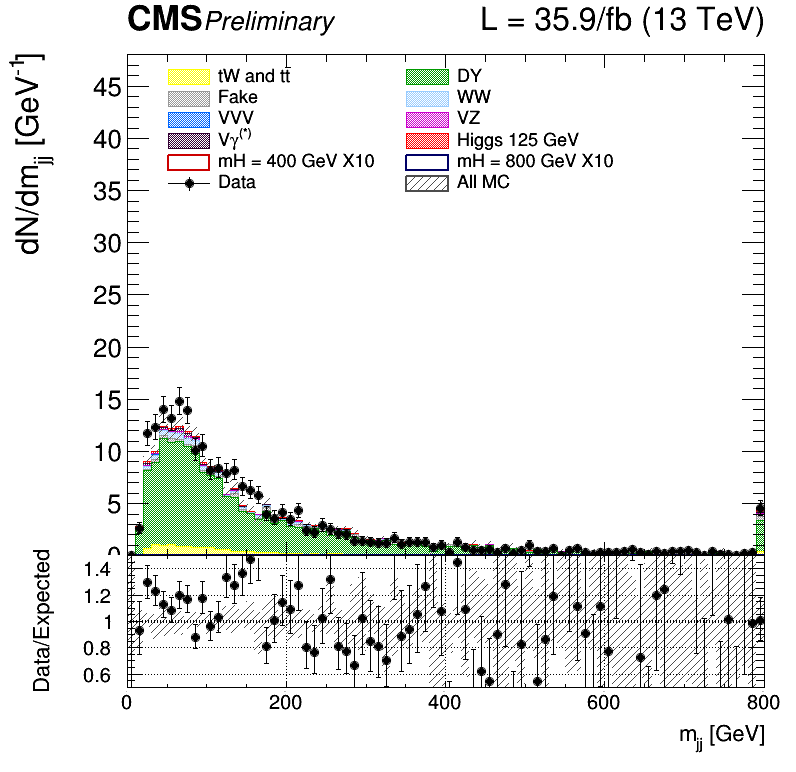
\includegraphics[width=0.45\textwidth]{Figs/OF_CR_Blind/cratio_hww2l2v_13TeV_dytt_of1j_mjj.png}
}                                              
\subfigure[$m_{\ell \ell}$]{                               
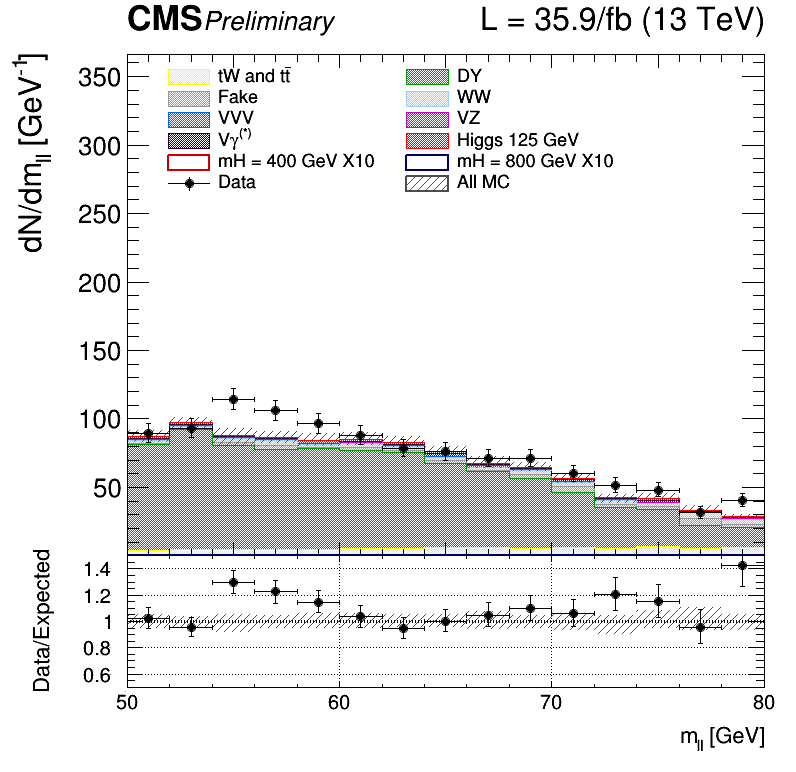
\includegraphics[width=0.45\textwidth]{Figs/OF_CR_Blind/cratio_hww2l2v_13TeV_dytt_of1j_mll_DY.png}
}\\

\subfigure[$p_T$ leading lepton]{                             
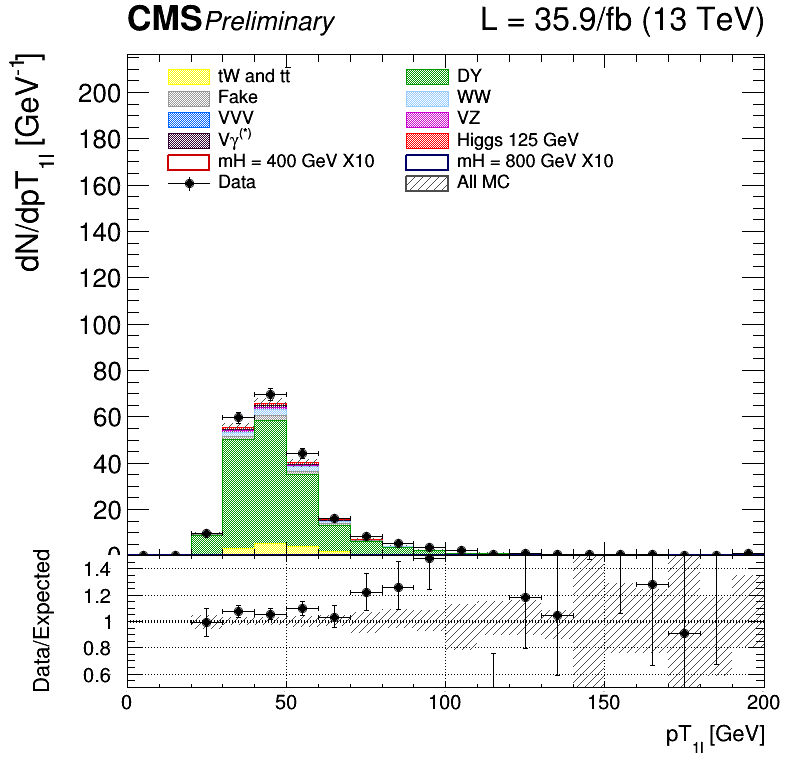
\includegraphics[width=0.45\textwidth]{Figs/OF_CR_Blind/cratio_hww2l2v_13TeV_dytt_of1j_std_vector_lepton_pt[0].png}
}                                              
\subfigure[$p_T^{\ell \ell}$]{                               
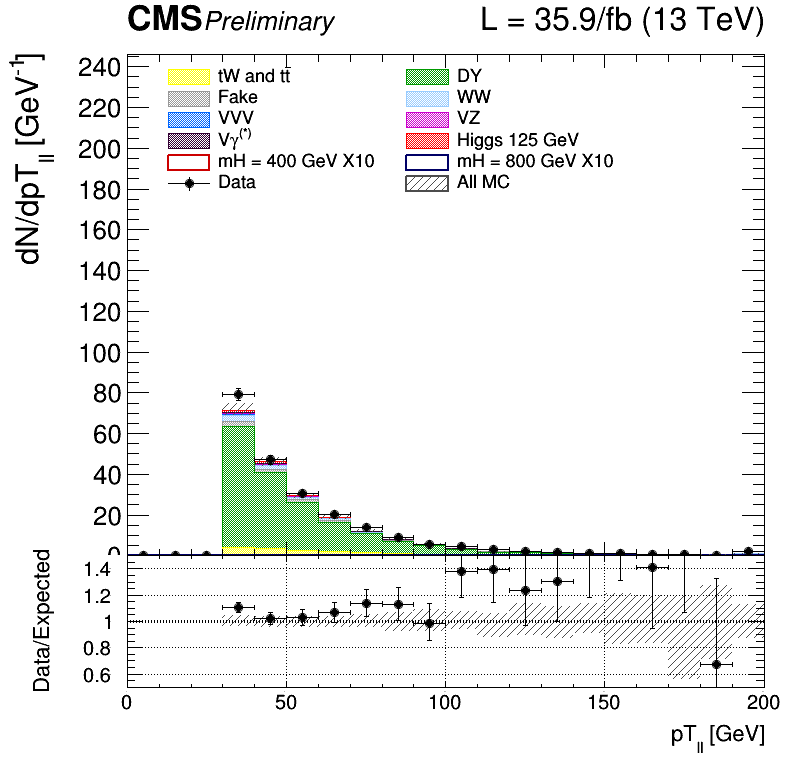
\includegraphics[width=0.45\textwidth]{Figs/OF_CR_Blind/cratio_hww2l2v_13TeV_dytt_of1j_ptll.png}
}\\

\caption{Control plots for several variables in a Drell-Yan enriched phase space for events with 1 jet.}
    \label{fig:CR_DY_OF_1}
\end{figure}





\begin{figure}[htbp]
\centering
\subfigure[$m_T^I$]{
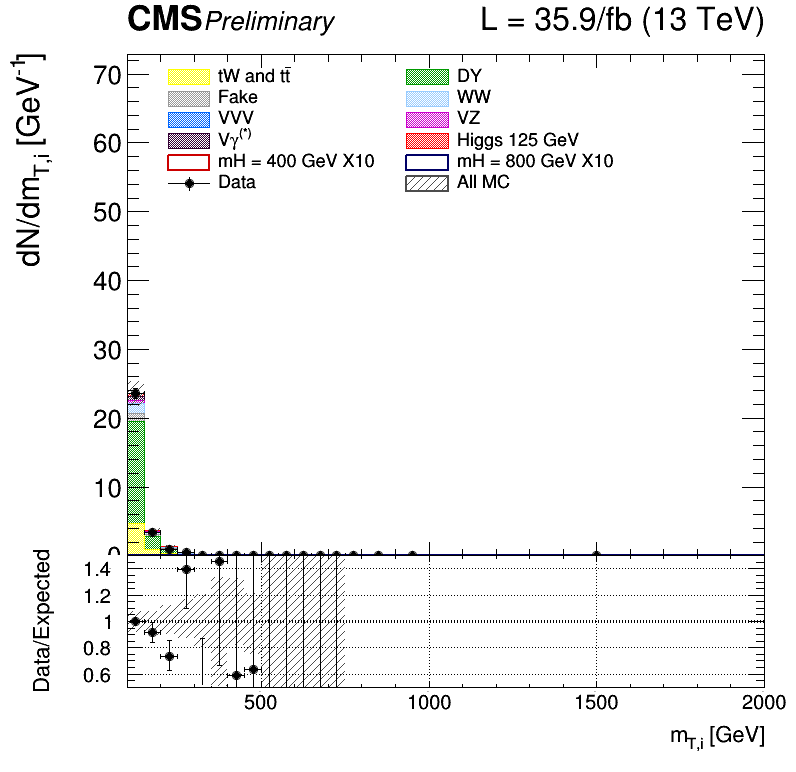
\includegraphics[width=0.45\textwidth]{Figs/OF_CR_Blind/cratio_hww2l2v_13TeV_dytt_of2j_mTi.png}
}
\subfigure[$m_T^H$]{
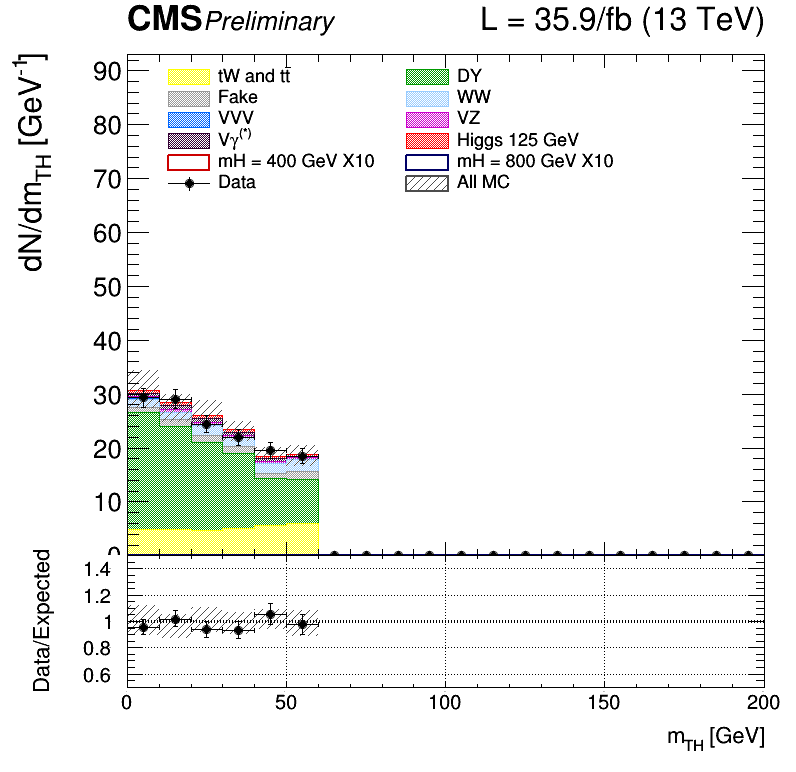
\includegraphics[width=0.45\textwidth]{Figs/OF_CR_Blind/cratio_hww2l2v_13TeV_dytt_of2j_mth_DY.png}
}                                              
\\                                             
\subfigure[$m_{jj}$]{                             
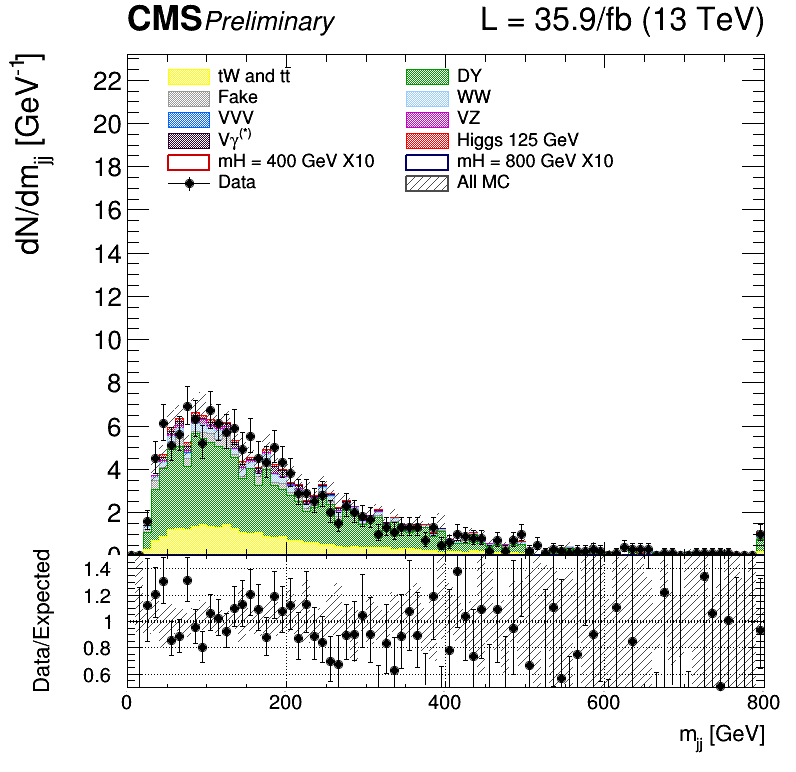
\includegraphics[width=0.45\textwidth]{Figs/OF_CR_Blind/cratio_hww2l2v_13TeV_dytt_of2j_mjj.png}
}                                              
\subfigure[$m_{\ell \ell}$]{                               
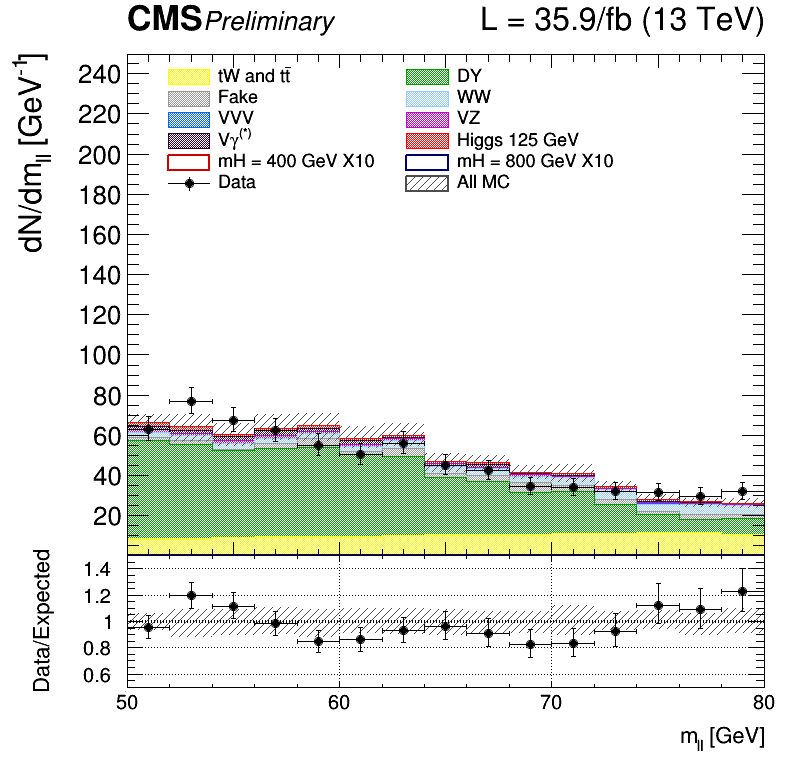
\includegraphics[width=0.45\textwidth]{Figs/OF_CR_Blind/cratio_hww2l2v_13TeV_dytt_of2j_mll_DY.png}
}\\

\subfigure[$p_T$ leading lepton]{                             
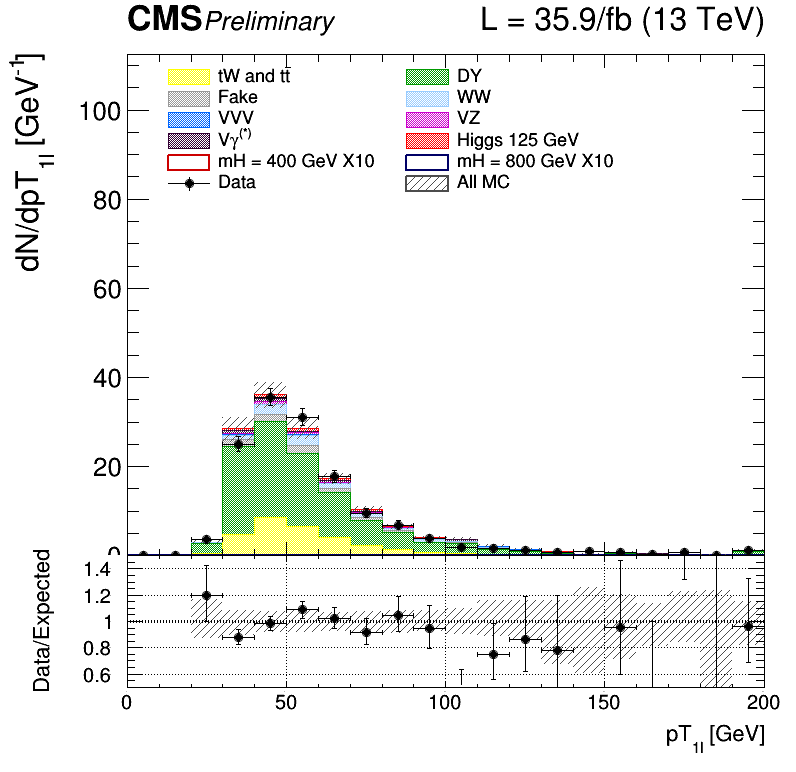
\includegraphics[width=0.45\textwidth]{Figs/OF_CR_Blind/cratio_hww2l2v_13TeV_dytt_of2j_std_vector_lepton_pt[0].png}
}                                              
\subfigure[$p_T^{\ell \ell}$]{                               
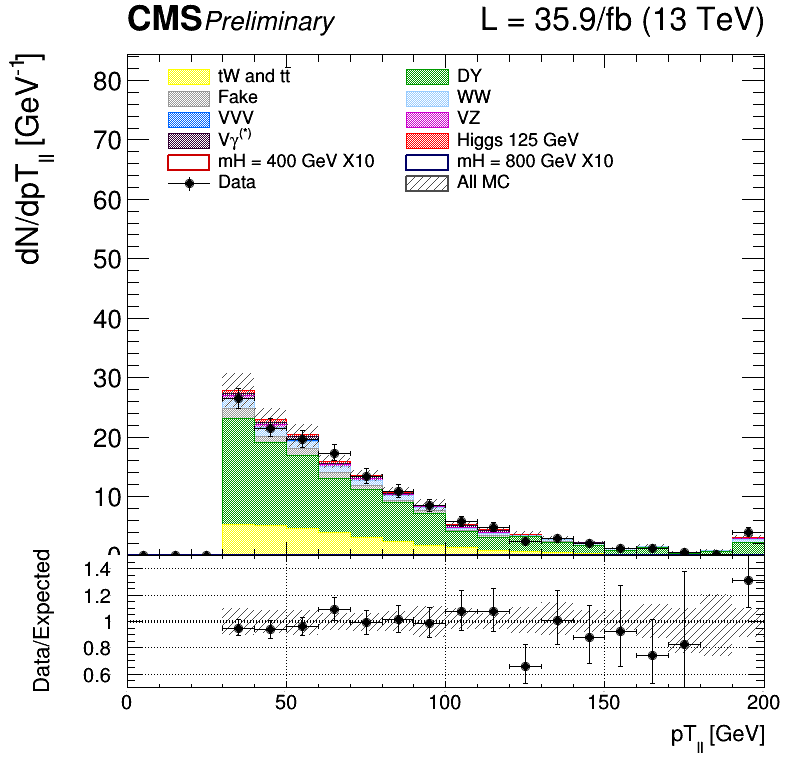
\includegraphics[width=0.45\textwidth]{Figs/OF_CR_Blind/cratio_hww2l2v_13TeV_dytt_of2j_ptll.png}
}\\

\caption{Control plots for several variables in a Drell-Yan enriched phase space for events with 2 jet.}
    \label{fig:CR_DY_OF_2}
\end{figure}




\begin{figure}[htbp]
\centering
\subfigure[$m_T^I$]{
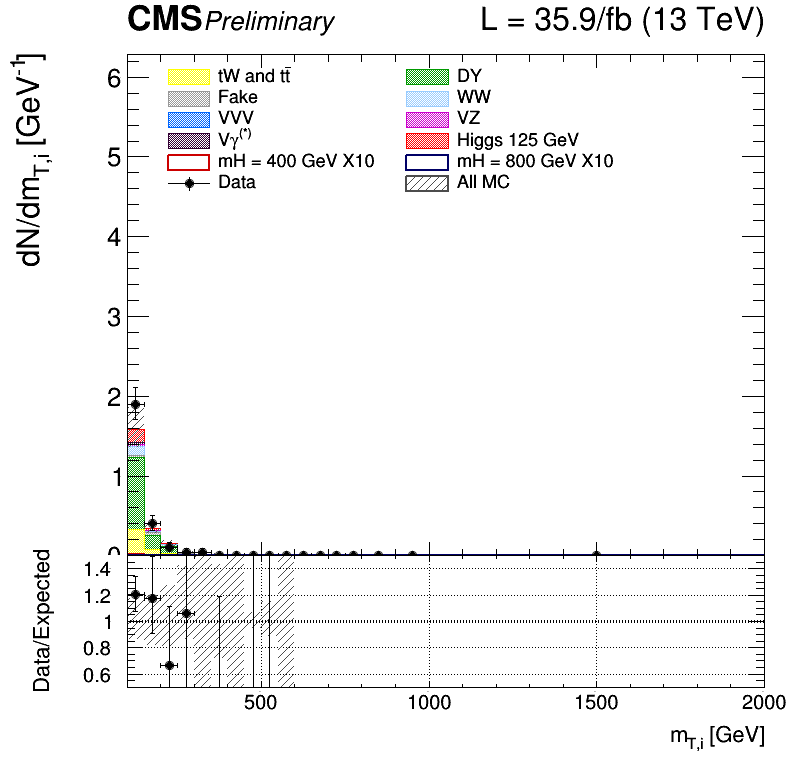
\includegraphics[width=0.45\textwidth]{Figs/OF_CR_Blind/cratio_hww2l2v_13TeV_dytt_of2j_vbf_mTi.png}
}
\subfigure[$m_T^H$]{
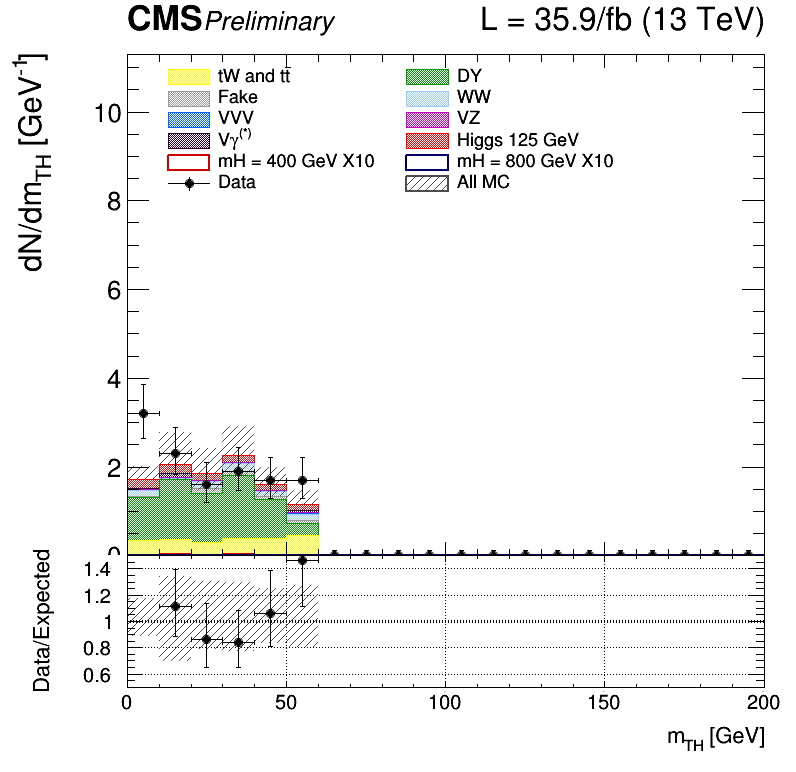
\includegraphics[width=0.45\textwidth]{Figs/OF_CR_Blind/cratio_hww2l2v_13TeV_dytt_of2j_vbf_mth_DY.png}
}                                              
\\                                             
\subfigure[$m_{jj}$]{                             
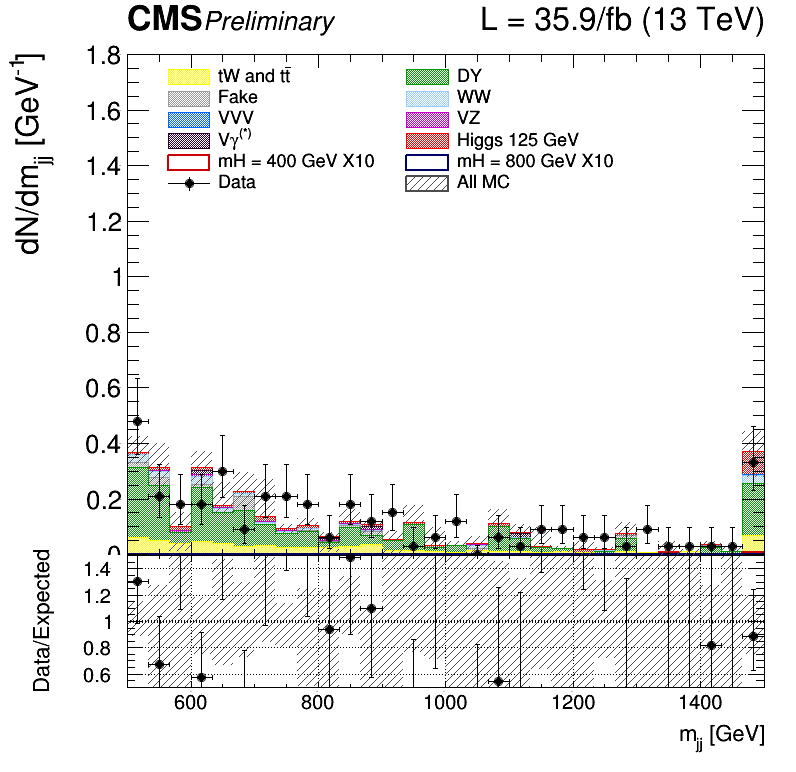
\includegraphics[width=0.45\textwidth]{Figs/OF_CR_Blind/cratio_hww2l2v_13TeV_dytt_of2j_vbf_mjj_DY_VBF.png}
}                                              
\subfigure[$m_{\ell \ell}$]{                               
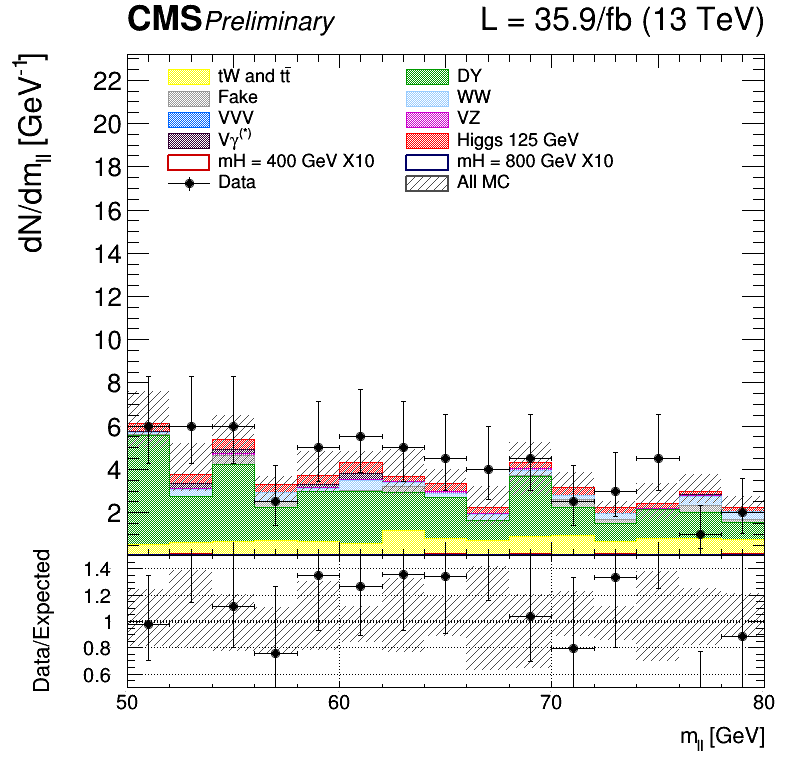
\includegraphics[width=0.45\textwidth]{Figs/OF_CR_Blind/cratio_hww2l2v_13TeV_dytt_of2j_vbf_mll_DY.png}
}\\

\subfigure[$p_T$ leading lepton]{                             
\includegraphics[width=0.45\textwidth]{Figs/OF_CR_Blind/cratio_hww2l2v_13TeV_dytt_of2j_vbf_std_vector_lepton_pt[0].png}
}                                              
\subfigure[$p_T^{\ell \ell}$]{                               
\includegraphics[width=0.45\textwidth]{Figs/OF_CR_Blind/cratio_hww2l2v_13TeV_dytt_of2j_vbf_ptll.png}
}\\

\caption{Control plots for several variables in a Drell-Yan enriched phase space for events for VBF.}
    \label{fig:CR_DY_OF_VBF}
\end{figure}







\newpage
\subsection{Top control region}
Similarly to the DY $\tau\tau$ case, control regions are defined for the top
background, and are used to normalize the top background to data.
The WW OF selection is used with inversion of the veto on b-jets. In
particular the following conditions are imposed to select a top enriched
control region for each of the 4 signal regions:
\begin{itemize}
\item {\bf 0 jet}, at least one b-tagged jet with 20 $< p_T <$ 30 GeV is required;
\item {\bf 1 jet}, exactly one b-tagged jet with $p_T$ above 30 GeV is required;
\item {\bf 2 jet}, exacly 2 jets with at least one of them b-tagged and in addition the condition $\Delta \eta_{jj} < 3.5$ {\bf or} $m_{jj} <$ 500 GeV;
\item {\bf VBF}, exacly 2 jets with at least one of them b-tagged and in addition the condition $\Delta \eta_{jj} > 3.5$ {\bf and} $m_{jj} >$ 500 GeV.
\end{itemize}
A jet is considered b-tagged if its cMVAv2 score is above the threshold
defining the loose working point.

The control plots for several variables in a top enriched phase space for events are shown in the Fig. below. The last bin in the distribution is the overflow.


\begin{figure}[htbp]
\centering
\subfigure[$m_T^I$]{
\includegraphics[width=0.45\textwidth]{Figs/OF_CR_Blind/cratio_hww2l2v_13TeV_top_of0j_mTi.png}
}
\subfigure[$m_T^H$]{
\includegraphics[width=0.45\textwidth]{Figs/OF_CR_Blind/cratio_hww2l2v_13TeV_top_of0j_mth.png}
}                                              
\\                                             
\subfigure[$m_{jj}$]{                             
\includegraphics[width=0.45\textwidth]{Figs/OF_CR_Blind/cratio_hww2l2v_13TeV_top_of0j_mjj.png}
}                                              
\subfigure[$m_{\ell \ell}$]{                               
\includegraphics[width=0.45\textwidth]{Figs/OF_CR_Blind/cratio_hww2l2v_13TeV_top_of0j_mll.png}
}\\

\subfigure[$p_T$ leading lepton]{                             
\includegraphics[width=0.45\textwidth]{Figs/OF_CR_Blind/cratio_hww2l2v_13TeV_top_of0j_std_vector_lepton_pt[0].png}
}                                              
\subfigure[$p_T^{\ell \ell}$]{                               
\includegraphics[width=0.45\textwidth]{Figs/OF_CR_Blind/cratio_hww2l2v_13TeV_top_of0j_ptll.png}
}\\

\caption{Control plots for several variables in the Top enriched phase space for events with 0 jet.}
    \label{fig:mll_sig}
\end{figure}




\begin{figure}[htbp]
\centering
\subfigure[$m_T^I$]{
\includegraphics[width=0.45\textwidth]{Figs/OF_CR_Blind/cratio_hww2l2v_13TeV_top_of1j_mTi.png}
}
\subfigure[$m_T^H$]{
\includegraphics[width=0.45\textwidth]{Figs/OF_CR_Blind/cratio_hww2l2v_13TeV_top_of1j_mth.png}
}                                              
\\                                             
\subfigure[$m_{jj}$]{                             
\includegraphics[width=0.45\textwidth]{Figs/OF_CR_Blind/cratio_hww2l2v_13TeV_top_of1j_mjj.png}
}                                              
\subfigure[$m_{\ell \ell}$]{                               
\includegraphics[width=0.45\textwidth]{Figs/OF_CR_Blind/cratio_hww2l2v_13TeV_top_of1j_mll.png}
}\\

\subfigure[$p_T$ leading lepton]{                             
\includegraphics[width=0.45\textwidth]{Figs/OF_CR_Blind/cratio_hww2l2v_13TeV_top_of1j_std_vector_lepton_pt[0].png}
}                                              
\subfigure[$p_T^{\ell \ell}$]{                               
\includegraphics[width=0.45\textwidth]{Figs/OF_CR_Blind/cratio_hww2l2v_13TeV_top_of1j_ptll.png}
}\\

\caption{Control plots for several variables in the Top enriched phase space for events with 1 jet.}
    \label{fig:mll_sig}
\end{figure}



\begin{figure}[htbp]
\centering
\subfigure[$m_T^I$]{
\includegraphics[width=0.45\textwidth]{Figs/OF_CR_Blind/cratio_hww2l2v_13TeV_top_of2j_mTi.png}
}
\subfigure[$m_T^H$]{
\includegraphics[width=0.45\textwidth]{Figs/OF_CR_Blind/cratio_hww2l2v_13TeV_top_of2j_mth.png}
}                                              
\\                                             
\subfigure[$m_{jj}$]{                             
\includegraphics[width=0.45\textwidth]{Figs/OF_CR_Blind/cratio_hww2l2v_13TeV_top_of2j_mjj.png}
}                                              
\subfigure[$m_{\ell \ell}$]{                               
\includegraphics[width=0.45\textwidth]{Figs/OF_CR_Blind/cratio_hww2l2v_13TeV_top_of2j_mll.png}
}\\

\subfigure[$p_T$ leading lepton]{                             
\includegraphics[width=0.45\textwidth]{Figs/OF_CR_Blind/cratio_hww2l2v_13TeV_top_of2j_std_vector_lepton_pt[0].png}
}                                              
\subfigure[$p_T^{\ell \ell}$]{                               
\includegraphics[width=0.45\textwidth]{Figs/OF_CR_Blind/cratio_hww2l2v_13TeV_top_of2j_ptll.png}
}\\

\caption{Control plots for several variables in the Top enriched phase space for events with 2 jet.}
    \label{fig:mll_sig}
\end{figure}



\begin{figure}[htbp]
\centering
\subfigure[$m_T^I$]{
\includegraphics[width=0.45\textwidth]{Figs/OF_CR_Blind/cratio_hww2l2v_13TeV_top_VBF_mTi.png}
}
\subfigure[$m_T^H$]{
\includegraphics[width=0.45\textwidth]{Figs/OF_CR_Blind/cratio_hww2l2v_13TeV_top_VBF_mth.png}
}                                              
\\                                             
\subfigure[$m_{jj}$]{                             
\includegraphics[width=0.45\textwidth]{Figs/OF_CR_Blind/cratio_hww2l2v_13TeV_top_VBF_mjj_DY_VBF.png}
}                                              
\subfigure[$m_{\ell \ell}$]{                               
\includegraphics[width=0.45\textwidth]{Figs/OF_CR_Blind/cratio_hww2l2v_13TeV_top_VBF_mll.png}
}\\

\subfigure[$p_T$ leading lepton]{                             
\includegraphics[width=0.45\textwidth]{Figs/OF_CR_Blind/cratio_hww2l2v_13TeV_top_VBF_std_vector_lepton_pt[0].png}
}                                              
\subfigure[$p_T^{\ell \ell}$]{                               
\includegraphics[width=0.45\textwidth]{Figs/OF_CR_Blind/cratio_hww2l2v_13TeV_top_VBF_ptll.png}
}\\

\caption{Control plots for several variables in the Top enriched phase space for events in VBF region.}
    \label{fig:mll_sig}
\end{figure}


